\documentclass[]{beamer}
\usepackage[spanish]{babel}
\usepackage{mathtools}
\usepackage{amsthm}
\usepackage{xcolor}
\usepackage[most]{tcolorbox} %para encerrar texto en cajas de colores

%%%% Mis macros %%%%

			%% Secciones:
	
			\newtheorem{teo}{\bf Theorem}
			\newtheorem{lema}{\textbf{Lemma}}
			\newtheorem{prop}{\bf Proposition}
			\newtheorem{obs}{\bf Observation}
			\newtheorem{dem}{\bf Proof}
			\newtheorem{cor}{\bf Corollary}
			\newtheorem{defi}{\bf Definition}
			\newtheorem{ej}{\bf Example}
			\newtheorem{notacion}{\bf Notation}
			\newtheorem{hip}{\bf Hypothesis}

			
			\theoremstyle{definition}
			\newtheorem{nota}{\bf Nota}

			%% Símbolos matemáticos
			\newcommand*{\QEDA}{\null\nobreak\hfill\ensuremath{\blacksquare}}%
			\newcommand*{\QEDB}{\null\nobreak\hfill\ensuremath{\square}}%
			\newcommand{\TODO}[1]{\textcolor{purple}{#1}}
			\newcommand*{\final}{\null\nobreak\hfill\ensuremath{\diamond}}
			\newcommand{\IR}{\mathbb{R}}
			\newcommand{\IC}{\mathbb{C}}
			\newcommand{\IN}{\mathbb{N}}
			\newcommand{\IZ}{\mathbb{Z}}
			\newcommand{\suma}[3]{\sum\limits_{#1}^{#2}#3} %Sumas y series
			\newcommand{\union}[3]{\bigcup\limits_{#1}^{#2}{#3}} %uniones
			\newcommand{\producto}[3]{\prod_{#1}^{#2}{#3}} %productos
			\newcommand{\limite}[2]{\lim\limits_{#1}{#2}} %límites
			\newcommand{\limsu}[2]{\lim\limits_{#1 \rightarrow \infty }#2_{#1}}
			%para límites de sucesiones
			\newcommand{\Om}{\Omega}
			\newcommand{\cali}[1]{\mathcal{#1}} %Letras caligráficas
			\newcommand{\cont}[2]{$\mathcal{C} [#1, #2]$}
			\newcommand{\integ}[3]{\int_{#1}^{#2}{#3}}
			\newcommand{\ldos}{\mathit{l}^{2}}


			\DeclareMathOperator*{\ameboxplus}{{\boxplus}}







\title{La transformada de Haar-Legendre}
\author{Amélie Bernès}

\usetheme{Madrid}
\useinnertheme{circles}

%\useoutertheme{sidebar} 

\title[PDL]{A study and spectral analysis of the discrete Legendre polynomials} 

\author{Amélie Bernès Carmona \and Moisés Soto Bajo} 

\institute[BUAP]{Benemérita Universidad Autónoma de Puebla \\ \smallskip \textit{ammel.bernes@gmail.com}}

\date[\today]{\today} % Presentation date or conference/meeting name, the optional parameter can contain a shortened version to appear on the bottom of every slide, while the required parameter value is output to the title slide

\begin{document}
\begin{frame}
\titlepage

\end{frame}

%----------------------------------------------------------



% Section; primera parte. Las subsections son
% Motivation and goals
% Construction of the BLD
% Symmetries
% Computation 
% Using representations with the BLD to perform a morphological analysis


%Section: segunda parte
% Motivation of doing a spectral analysis
% Spectral analysis with the DFT
% Spectral analysis using monofrecuential spaces
%
%----------------------------------------------------------
\section{Primera parte}

\begin{frame}
\Huge{
\textbf{
Motivation
}}
\end{frame}


\begin{frame}
Fixed $n \geq 2$, a signal of dimension $n$ will be represented
with a vector of $\IR^{n}$.

\begin{figure}[h]
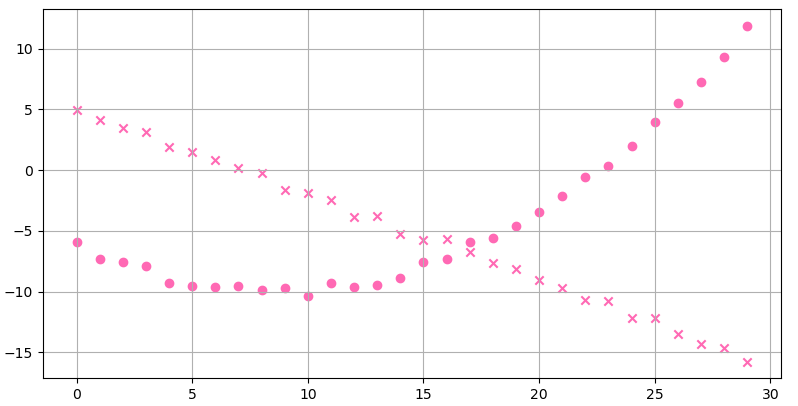
\includegraphics[scale = 0.4]{a}
\end{figure}
We are interested in geometric attributes of the signal, particularly, in
knowing when it behaves like a straight line or like a parabola.

\[
G_{x} := \{ (m, x_{m}) : \hspace{0.2cm} 0 \leq m \leq n-1 \}.
\]

\textbf{Constant, affine and quadratic signals.}
\end{frame}


\begin{frame}
\Huge{
\textbf{
Part One: Definition of the discrete Legendre polynomials
}}
\end{frame}



\begin{frame}
\subsection{Motivation and goals}
Fixed a dimension $n \geq 2$, we are looking for a
basis $$\cali{L}^{n} = \{\cali{L}^{n,k}: \hspace{0.2cm}
0 \leq k \leq n-1\}$$ of $\IR^{n}$ such that
\begin{itemize}
	\item \textcolor{red}{(Size)}
	It is an orthonormal basis of $\IR^{n}$;
\end{itemize}
\[
\forall x\in \IR^{n}: \hspace{0.2cm} x = \suma{k=0}{n-1}{
\langle x, \cali{L}^{n,k} \rangle
}
\]
and
\[
\forall x\in \IR^{n}: \hspace{0.2cm} || x ||^{2} = \suma{k=0}{n-1}{
| \langle x, \cali{L}^{n,k} \rangle |^{2}
}
\]
\begin{itemize}
	\item \textcolor{red}{(Shape)}
	It's possible to establish a simple criteria 
	for the shape of the graph of any signal $x$	
	in terms
	of the coefficients  
	$\langle x, \cali{L}^{n,k} \rangle$ of it with respect
	to $\cali{L}^{n}$.
\end{itemize}


\end{frame}
%----------------------------------------------------------


\begin{frame}
\frametitle{Basic definitions and notations}
Let $n \geq 2$.
\begin{itemize}
	\item For all $f \in \IR[t]$ and uniform mesh
	$\cali{P} = \{ t_{j} := t_{0}+ hj : 
	\hspace{0.2cm} 0 \leq j \leq n-1 \}$ of $n$ points, we define
	\[
	\Omega_{n, \cali{P}}(f) := (f(t_{j}))_{j=0}^{n-1} \in \IR^{n}
	\]
	\item For all $0 \leq k \leq n-1$, let
	\[
	v_{k} := \Omega_{n, \cali{P}}(f_{k}),
	\]
	where $f_{k} = t^{k}$.
	\item For all $0 \leq k \leq n-1$, let
	\[
	W_{k} := span \{ v_{j} : \hspace{0.2cm} 0 \leq j \leq k \} \leq \IR^{n}
	\]
\end{itemize}
\end{frame}


\begin{frame}
\frametitle{Key proposition}
\begin{prop}
Let $n \geq 2$ and $\cali{P} = \{ t_{j} := t_{0}+ hj : 
	\hspace{0.2cm} 0 \leq j \leq n-1 \}$ be a uniform mesh 
	of $n$ points. If $f(t) \in \IR[t]$ is a polynomial
	of degree less than $n$ and $\Omega_{n, \cali{P}}(f)$
	is the zero vector, then $f$ is the zero polynomial.
\end{prop}

Reason: $\Omega_{n, \cali{P}}(f) = 0$ iff
all the $n$ elements of the mesh $\cali{P}$ are roots of $f$. \\

It is just a simple consequence of the Fundamental
Theorem of Algebra, yet we use it widely in our arguments.
\end{frame}


\begin{frame}
\frametitle{Using the operator $\Omega_{n, \cali{P}}$ to reformulate geometric properties}
Let $x = (x_{m})_{m=0}^{n-1} \in \IR^{n}$.
\begin{align*}
x \textit{ is affine}  \Leftrightarrow &
x = (a + bi)_{i=0}^{i} \hspace{0.2cm} \textit{for some } a, b \in \IR \\
\Leftrightarrow & x = \Omega_{n, \cali{P}_{n}}(l(t)) \textit{for some } l(t) = a+bt \in \IR_{1}[t] \\
\Leftrightarrow & x = a w_{0} + bw_{1} \\
\Leftrightarrow & x \in W_{n, 1}.
\end{align*}
Likewise, 
\begin{center}
$x$ is constant iff $x \in W_{n,0}$
\end{center}
and
\begin{center}
$x$ is cuadratic iff $x \in W_{n,2}$.
\end{center}
\end{frame}

\begin{frame}
\frametitle{Some properties of the subspaces $W_{n,k}$}
\section{Some properties of the subspaces $W_{n,k}$}
\begin{prop}
		Let $n \geq 2$, $0 \leq k \leq n-1$. Let $W_{n,k}$
		be as.
		\begin{itemize}
		\item $dim(W_{n,k}) = k+1$, 
		\item $\forall 0 \leq i \leq n-2$: $W_{n, i} \subseteq W_{n, i+1}$,
		\item $\IR^{n} = W_{n, n-1}$
		\item Let $\cali{P}$ be a uniform mesh of $n$
		points. For all $x \in \IR^{n}$ and all $0 \leq i \leq n-1$, $x \in W_{n,i}$
		if and only if there exists a polynomial $g(x)$ of degree at most
		$i$ such that $x = \Omega_{n, \cali{P}}(g)$.
		\end{itemize}
\end{prop}
\end{frame}



\begin{frame}

The \textbf{belonging }to a subspace $W_{n,k}$
determines the \textbf{shape} of the graph of a signal $x$.

\begin{figure}[h]
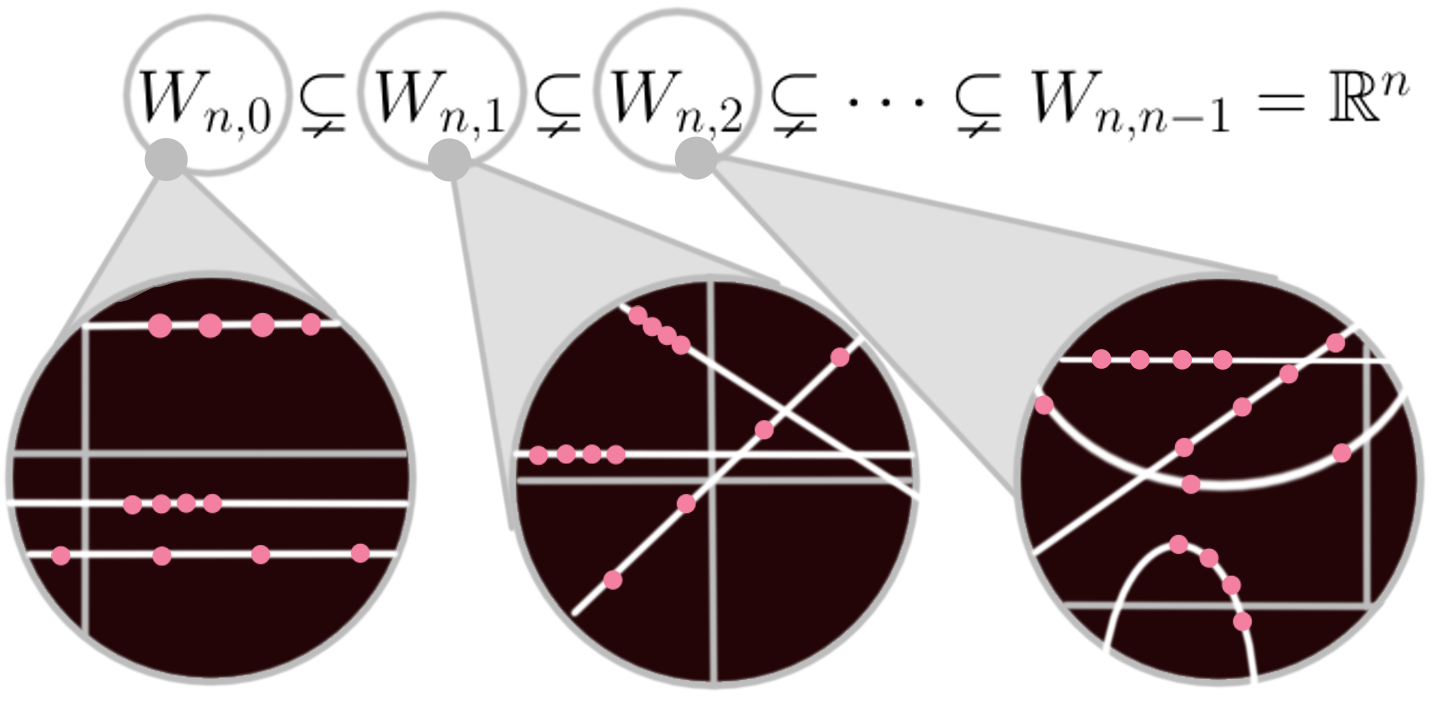
\includegraphics[scale = 1]{nuevas_lupas}
\end{figure}
\end{frame}


\begin{frame}
\frametitle{The definition of the degree of a finite signal}


\begin{prop}
Let $n \geq 2$ and $\cali{P}$ be a uniform mesh of $n$ points.
The function 
\[
\Omega_{n, \cali{P}}: \IR_{n-1}[t] \longrightarrow \IR^{n}
\]
is an isomorphism of $\IR-$vector spaces.
\end{prop}

Notice that the mesh $\cali{P}$ is fixed at the beginning. \\

\textbf{Question:}
Can we find two uniform meshes $\cali{P}$ and $\tilde{\cali{P}}$
and two polynomials $f, \tilde{f}$ of degrees
$0 \leq \partial(f) < \partial(\tilde{f}) \leq n-1$
such that
\[
\Omega_{n, \cali{P}}(f) = x = \Omega_{n, \tilde{\cali{P}}}(\tilde{f}) ?
\]
\end{frame}

\begin{frame}
What is certain is that we can not assure uniqueness if
we remove the restriction in the degrees of the polynomials. 
\begin{figure}[h]
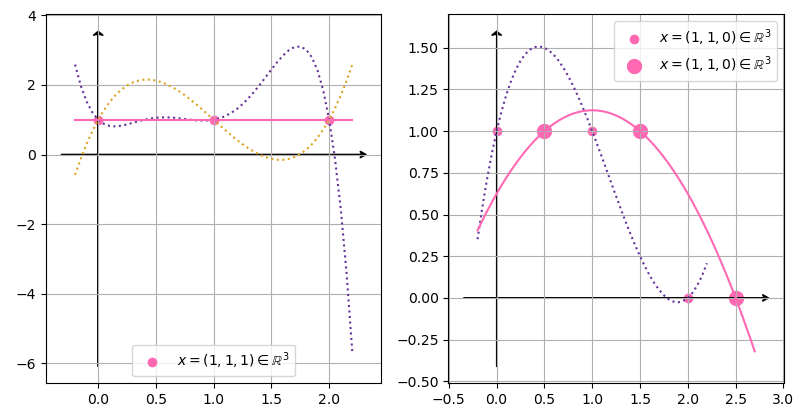
\includegraphics[scale = 0.5]{25Nov_1}
\end{figure}
\end{frame}

\begin{frame}
\begin{prop}
Let $n \geq 2$, $x \in \IR^{n}$. If $\cali{P}$ and $\tilde{\cali{P}}$
are uniform meshes of $n$ points and $f, \tilde{f} \in \IR_{n-1}[t]$ 
are such that
\[
\Omega_{n, \cali{P}}(f) = x = \Omega_{n, \tilde{\cali{P}}}(\tilde{f}).
\]
then $\partial(f) = \partial(\tilde{f})$.
\end{prop}

\begin{defi}
Let $n \geq 2$ and $x \in \IR^{n}$. If $f \in \IR_{n-1}[t]$
and $\cali{P}$ is a uniform mesh of $n$ points such that
$x = \Omega_{n, \cali{P}}(f)$, then 
\[
\partial(x) := \partial(f)
\]
\end{defi}
\end{frame}


\begin{frame}
\frametitle{Thus, $W_{n,k}$ is the space of signals of degree $k$. }

\begin{teo}
Let $n \geq 2$ and $x \in \IR^{n}$.
\begin{itemize}
\item $x$ has degree 0 iff $x \in W_{n,0}$
\item for all $1 \leq i \leq n-1$, $x$ has degree $i$ iff
$x \in W_{n,i}$
\end{itemize}
\end{teo}

Thus, if $x \in \IR^{n}$, 
\begin{itemize}
	\item The graph of $x$ has the shape of a polynomial
	of degree $k$ if and only if $x \in W_{n,k}$
	(binary answer)
	\item We can actually measure how far apart 
	$x$ is from $W_{n,k}$, thus \textbf{we can measure how much
	$x$ is far away from the property ``having degree $k$''}
\end{itemize}

Let's find orthonormal basis for the spaces $W_{n,k}$.

\end{frame}


\begin{frame}
\frametitle{Finding orthonormal basis for $W_{n,k}$}
\begin{figure}[h]
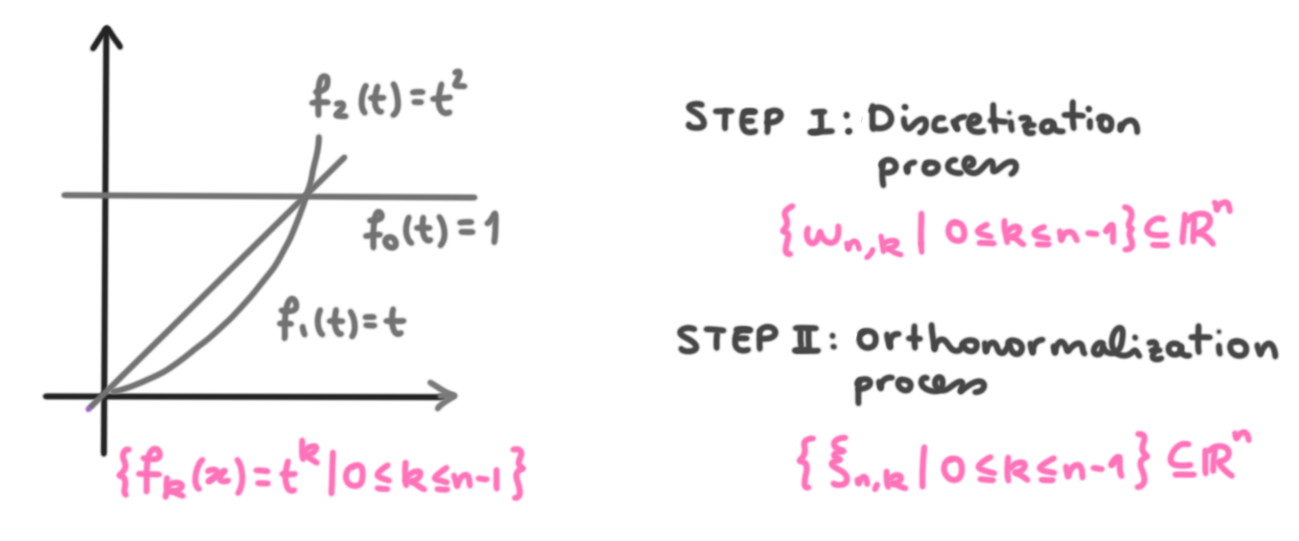
\includegraphics[scale = 1]{1}
\end{figure}
\end{frame}

\begin{frame}
\begin{figure}[h]
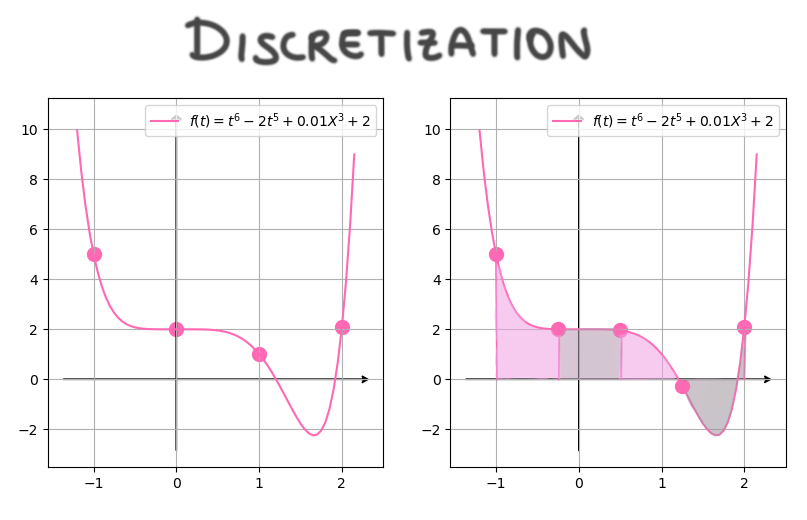
\includegraphics[scale = 1.4]{discretization}
\end{figure}
\end{frame}

\begin{frame}
\begin{figure}[h]
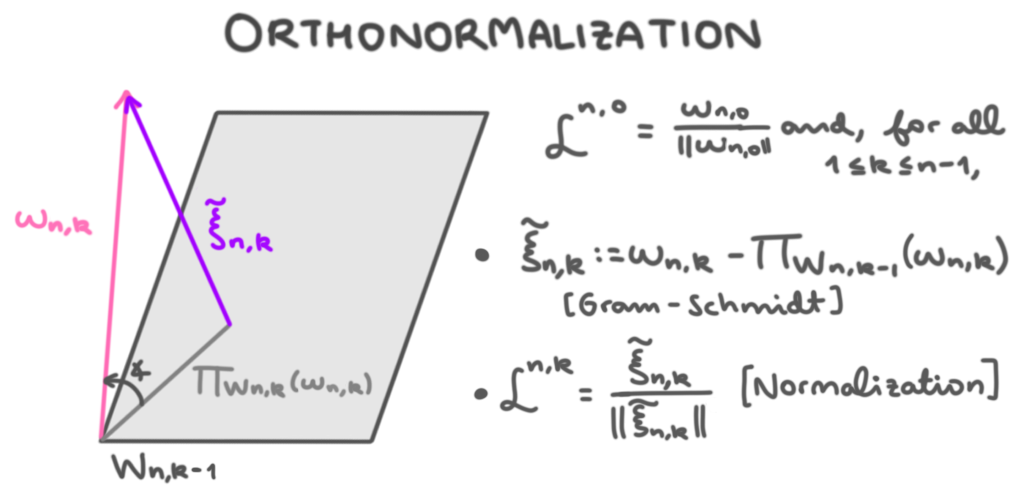
\includegraphics[scale = 1.4]{orthonorm}
\end{figure}
\end{frame}

\begin{frame}
\frametitle{The Discrete Legendre basis}
Since $W_{n, n-1} = \IR^{n}$, 
\[
\cali{L}^{n} := \{ \cali{L}^{n,k}: \hspace{0.2cm} 0 \leq k \leq n-1 \}
\]
is an orthonormal basis for $\IR^{n}$. We call it the
\textbf{discrete Legendre basis of dimension $n$}.
\end{frame}


\begin{frame}
\frametitle{How to measure the distance to a subspace?}
\begin{figure}[h]
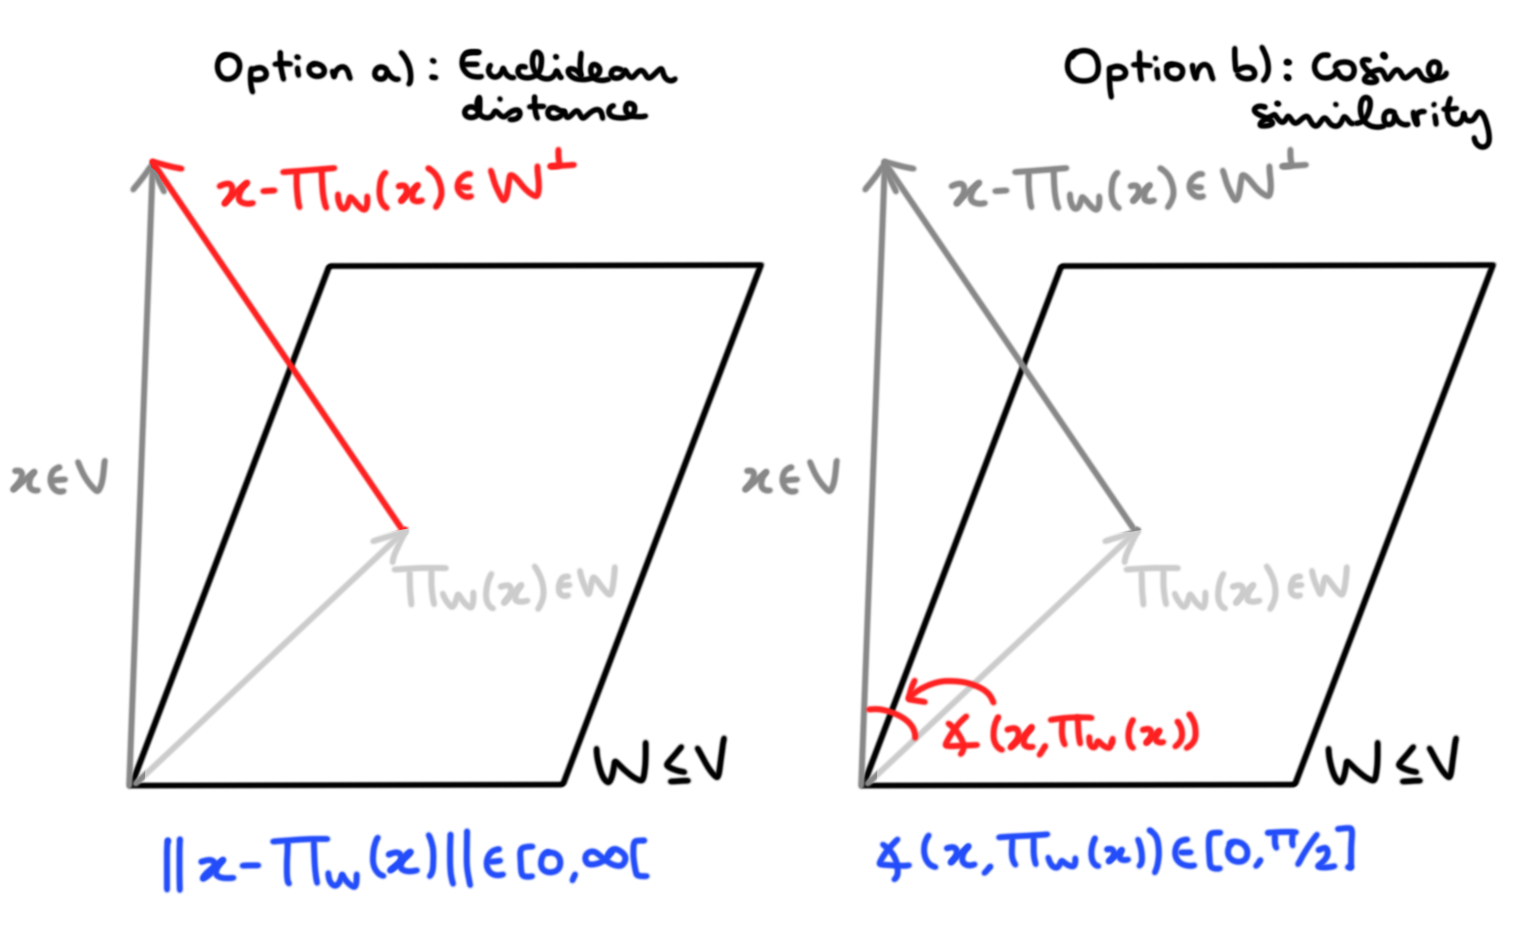
\includegraphics[scale = 0.9]{18Sept_1}
\end{figure}
\end{frame}

\begin{frame}
\frametitle{Why cosine similarity is better for us?}
Answer: it is, as well as the
shape of the graph of a signal, 
invariant under scalar multiplication.

\begin{figure}[h]
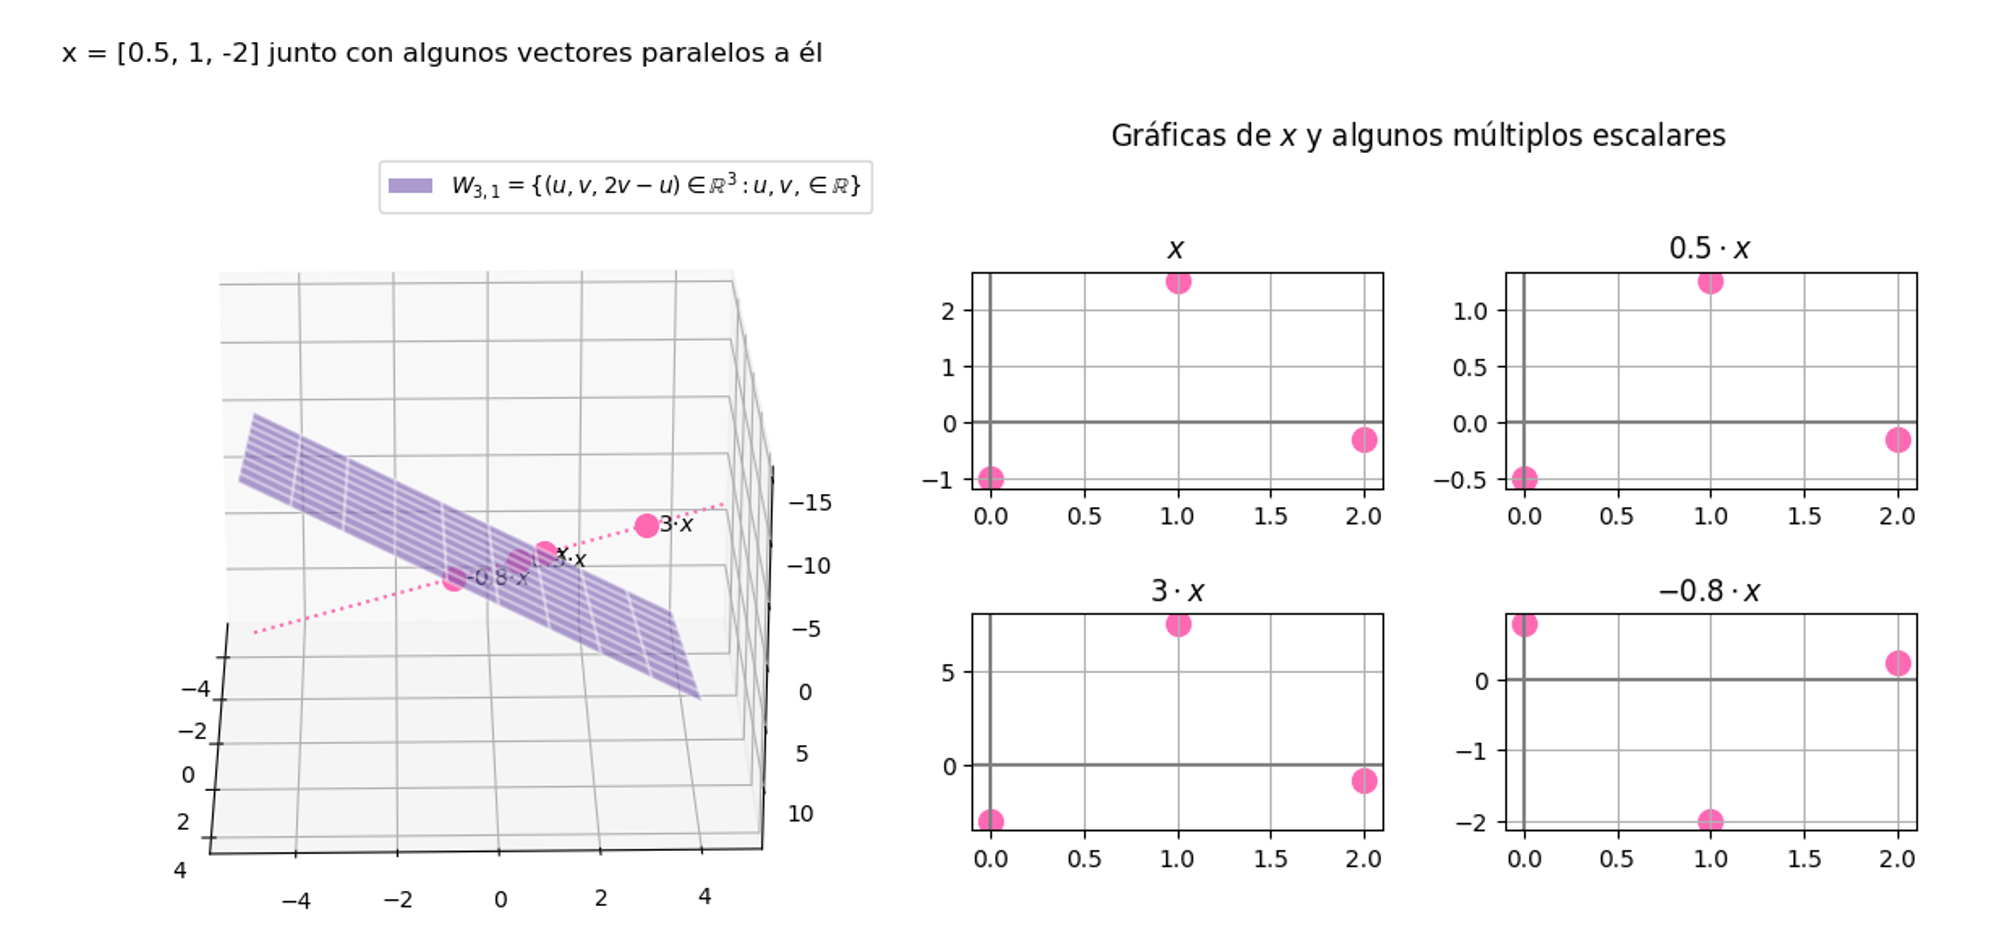
\includegraphics[scale = 0.15]{borrador}
\end{figure}
\end{frame}


\begin{frame}
\frametitle{Using coefficientes with respect to $\cali{L}^{n}$ to make a morphological analysis}
\begin{figure}[h]
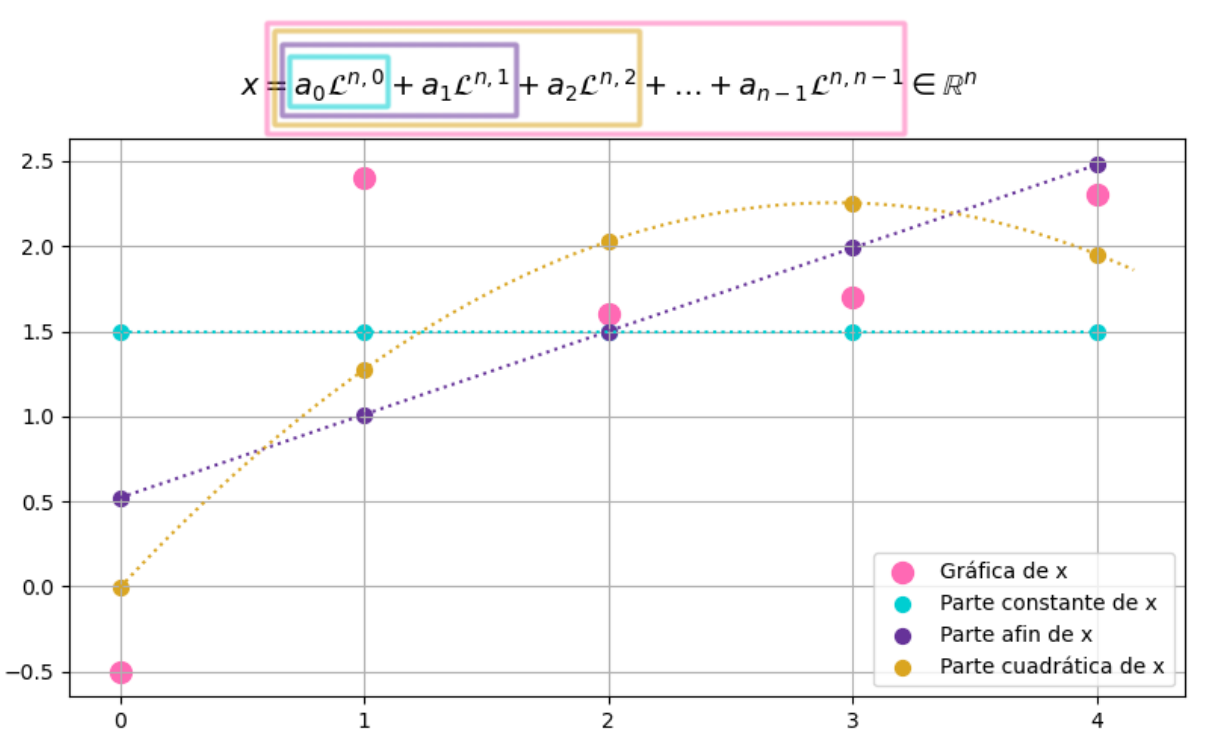
\includegraphics[scale = 0.35]{abee}
\end{figure}
\end{frame}



\begin{frame}
Let $x = \suma{i=0}{n-1}{a_{i}\cali{L}^{n,i}} \in \IR^{n}$.
Of course, $a_{i} := \langle x, \cali{L}^{n,i} \rangle$.
\begin{itemize}
	\item $x$ is approximately constant iff $a_{0}^{2} \sim ||x||^{2}$ 
	\item $x$ is approximately affine iff $a_{0}^{2} + a_{1}^{2} \sim ||x||^{2}$ 
	\item $x$ is approximately quadratic iff $a_{0}^{2} + a_{1}^{2} + a_{2}^{2} \sim ||x||^{2}$ 
\end{itemize}

In general, \textbf{$x$ has nearly degree $k$ iff the energy 
$||x||^{2}$ of the signal
is concentrated in the first $k$ coefficients $a_{k}$.}
\end{frame}



\begin{frame}
\frametitle{Formulas for computing the cosine similarity to the spaces $W_{n,k}$}
\begin{minipage}{0.5\textwidth}
If $x = \suma{i=0}{n-1}{a_{i} \cali{L}^{n,k}}$, then
\[
||x||^{2} = \suma{i=0}{n-1}{a_{i}^{2} \cali{L}},
\]
\[
||\Pi_{W_{n,k}}(x)||^{2} = \suma{i=0}{k}{a_{i}^{2} \cali{L}},
\]
\[
||\Pi_{W_{n,k}^{\perp}}(x)||^{2} = \suma{i=k+1}{n-1}{a_{i}^{2} \cali{L}}.
\]

\end{minipage} \hfill
\begin{minipage}{0.45\textwidth}

\begin{figure}[h]
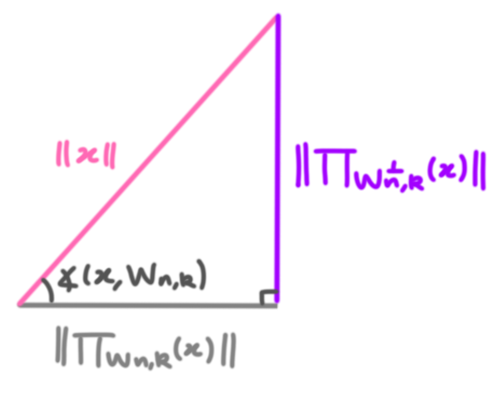
\includegraphics[scale = 0.4]{4Jun23_1}
\end{figure}

\end{minipage}
\end{frame}


\begin{frame}
Thus, if $x = \suma{i=0}{n-1}{a_{i} \cali{L}^{n,k}}$,
\[
cos(\measuredangle(x, W_{n,k})) = \sqrt{
\frac{
\suma{i=0}{k}{a_{i}^{2} \cali{L}}
}{
\suma{i=0}{n-1}{a_{i}^{2} \cali{L}}}
} \in [0,1]
\]
is a measure of how near $x$ is to the property of having the
shape of a polynomial of degree $k$.
\end{frame}



\begin{frame}
\frametitle{Example in $\IR^{3}$}
Notice that $W_{3,1}$ is an hyper-plane of $\IR^{3}$.
\begin{figure}[h]
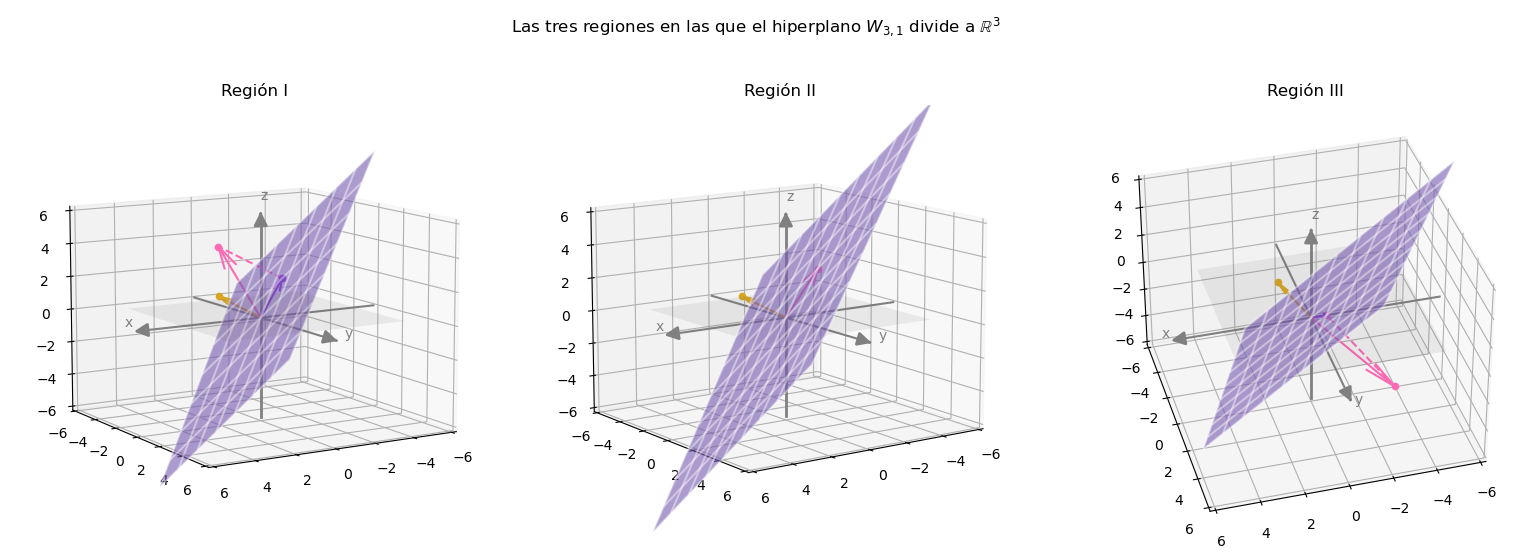
\includegraphics[scale = 0.3]{2Dic_4}
\end{figure}
\end{frame}

\begin{frame}
\begin{figure}[h]
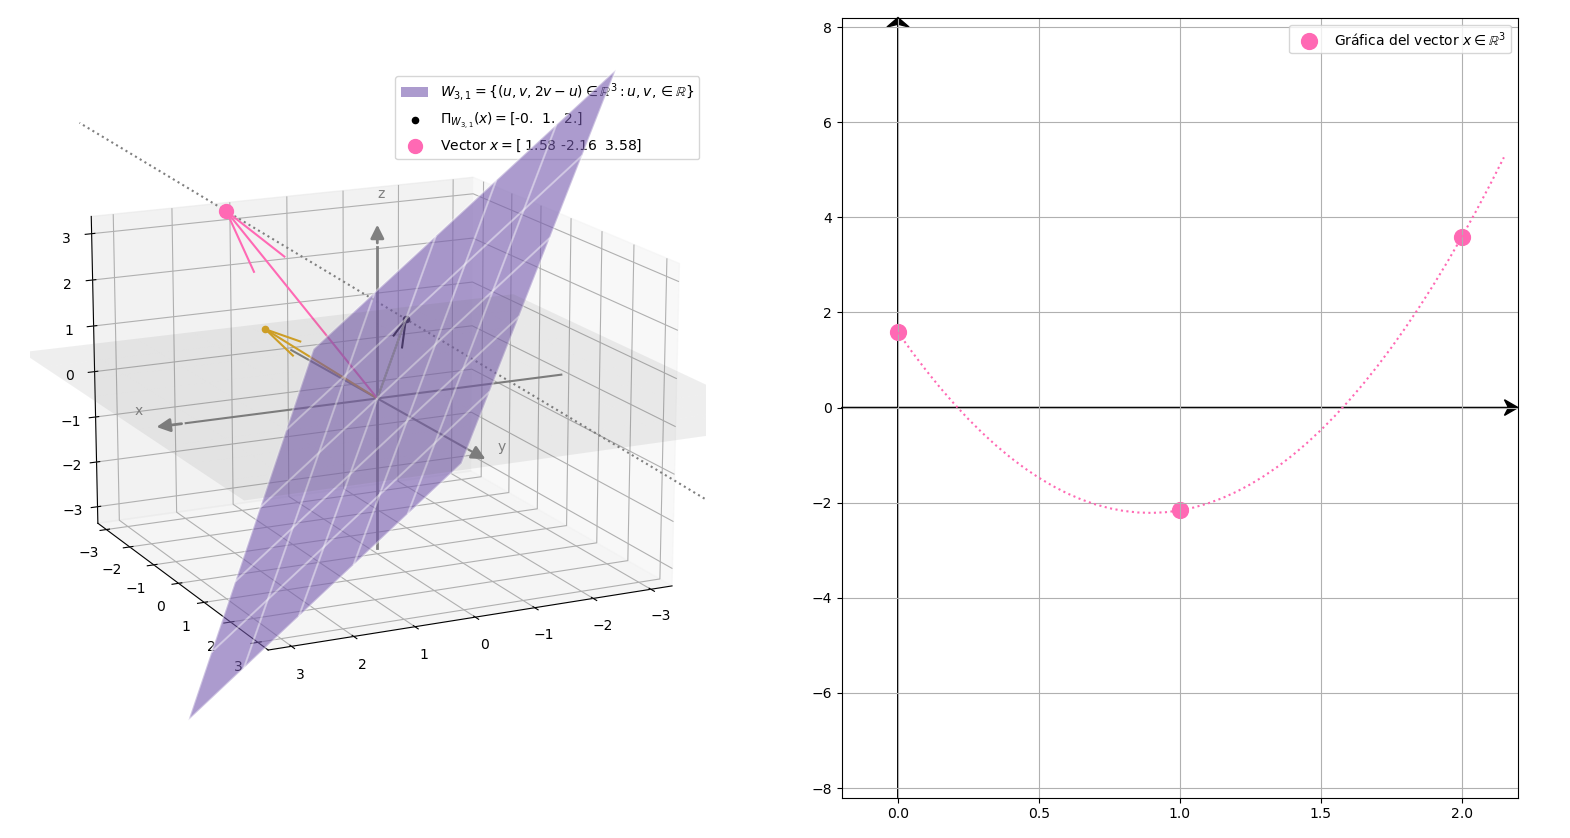
\includegraphics[scale = 0.3]{6Dic_0}
\end{figure}
\end{frame}

\begin{frame}
\begin{figure}[h]
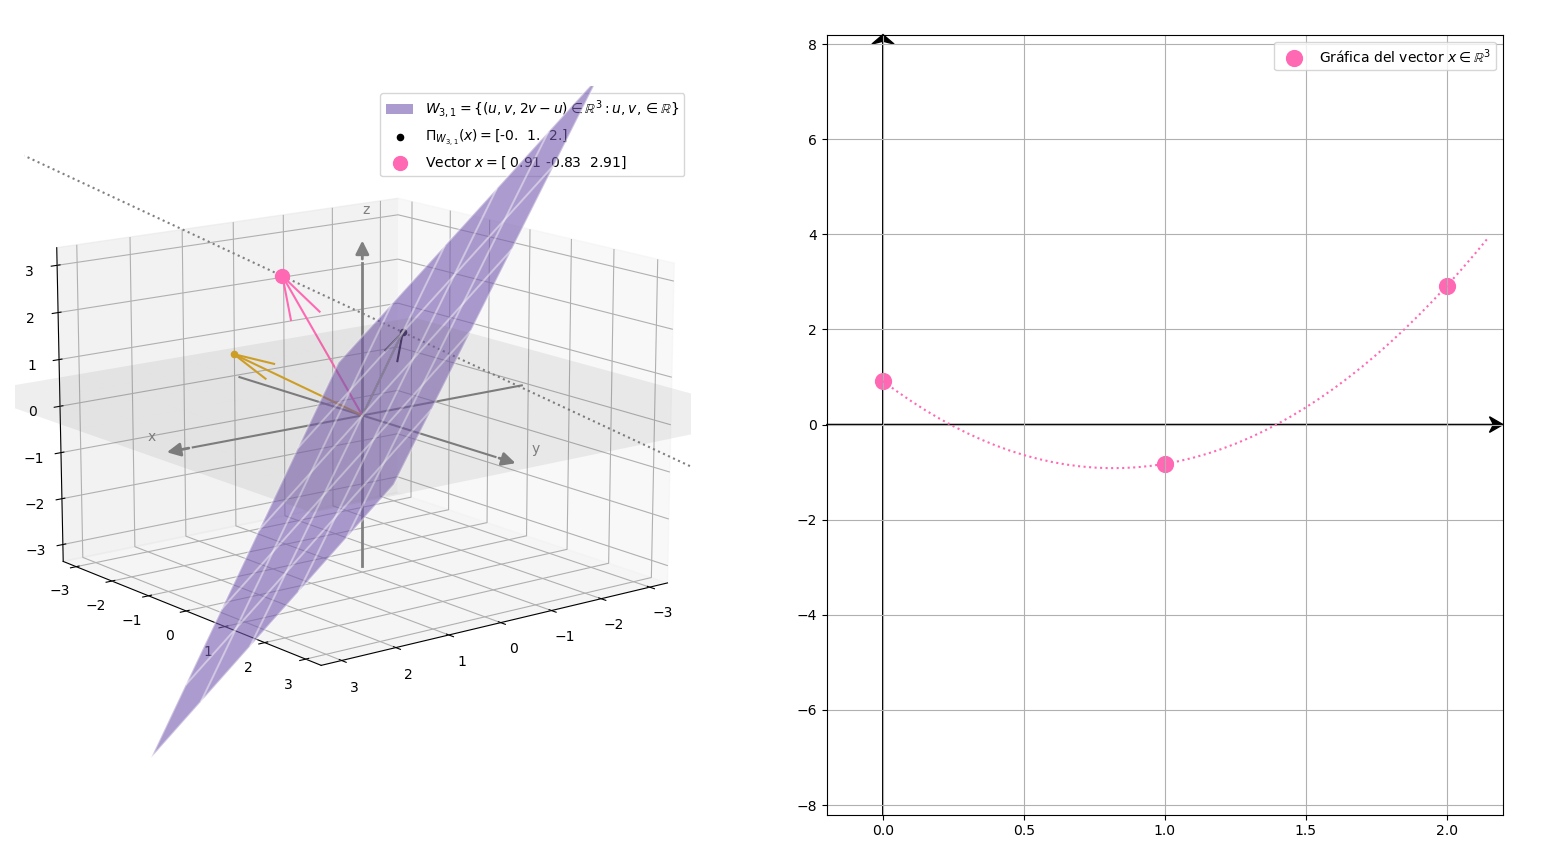
\includegraphics[scale = 0.3]{6Dic_1}
\end{figure}
\end{frame}

\begin{frame}
\begin{figure}[h]
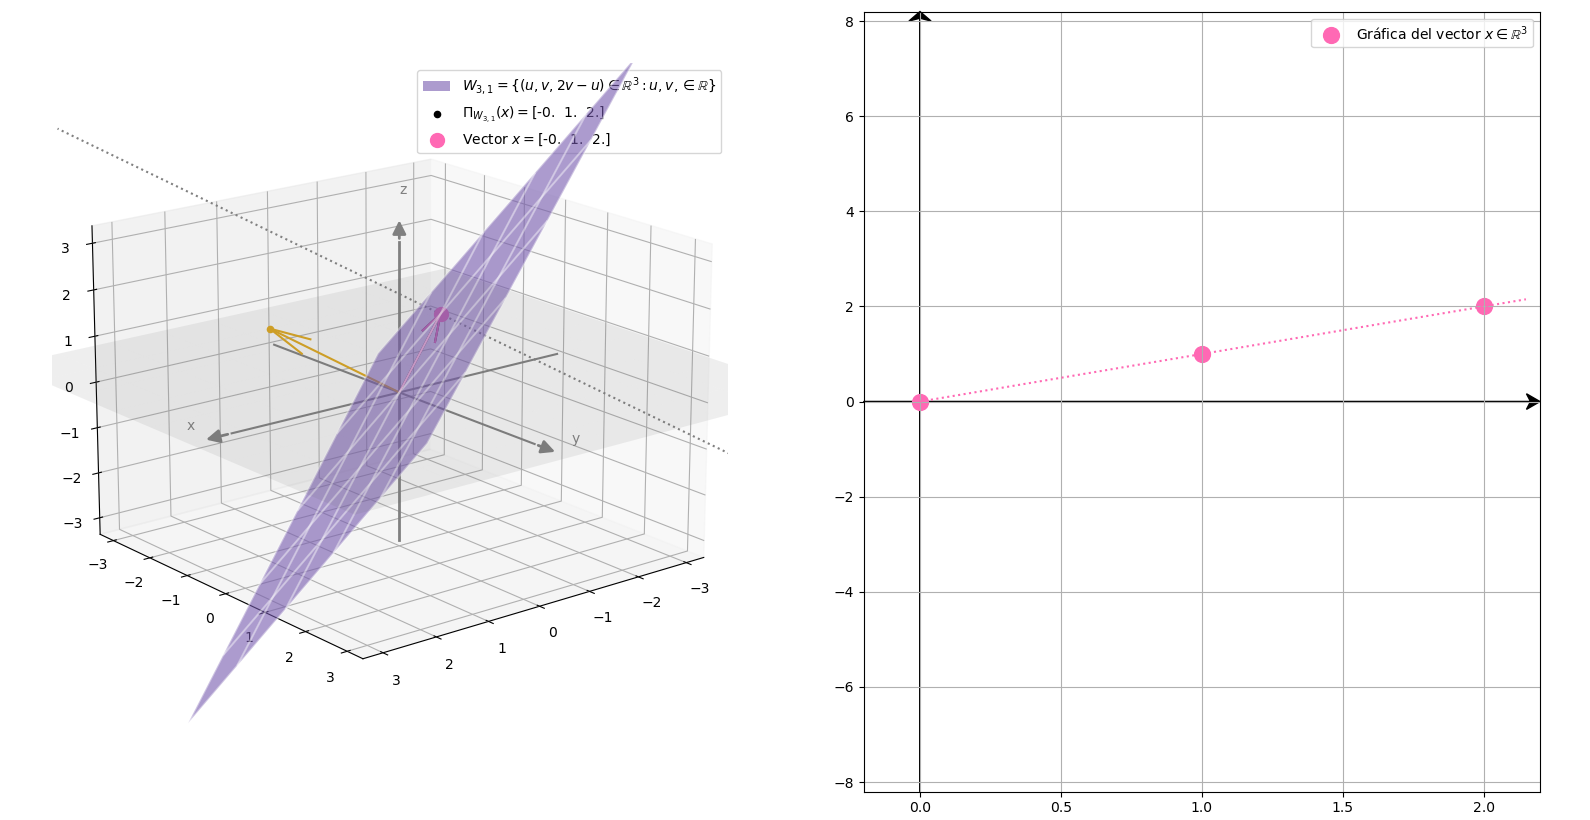
\includegraphics[scale = 0.3]{6Dic_2}
\end{figure}
\end{frame}

\begin{frame}
\begin{figure}[h]
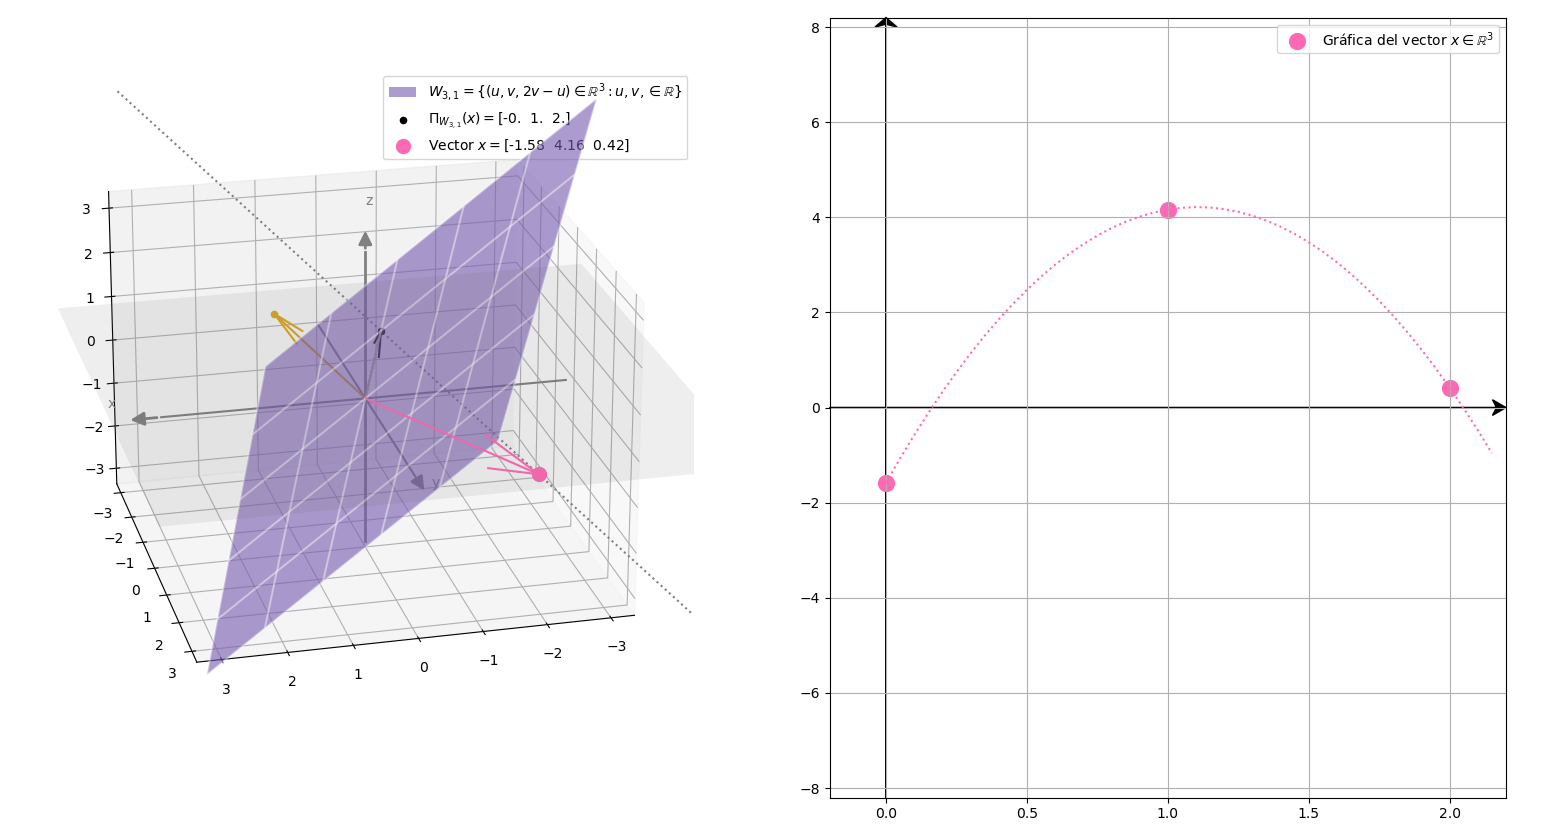
\includegraphics[scale = 0.3]{6Dic_3}
\end{figure}
\end{frame}

\begin{frame}
\begin{figure}[h]
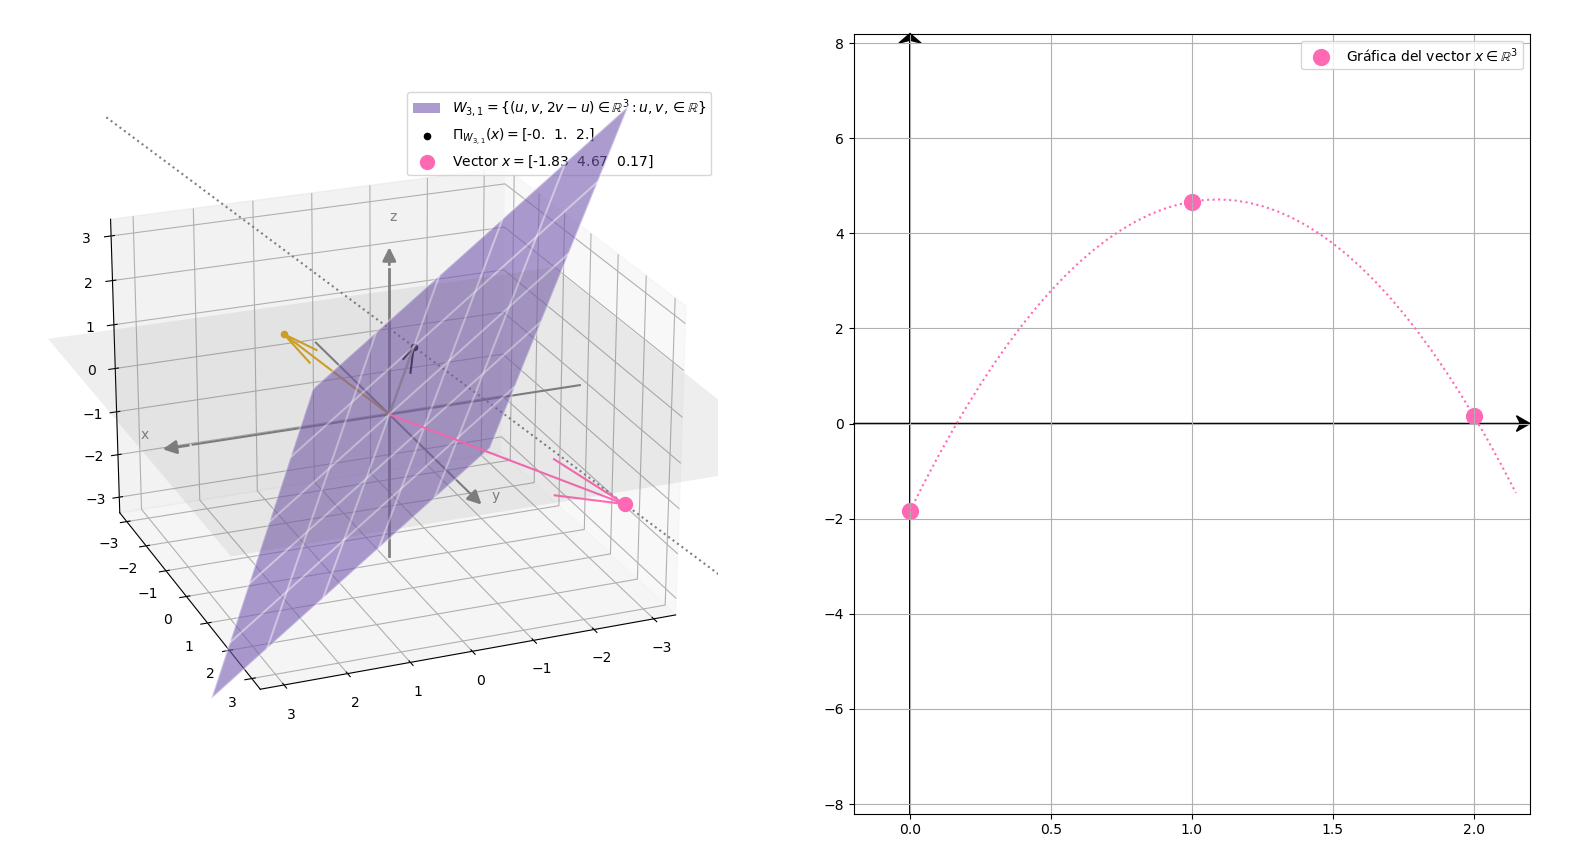
\includegraphics[scale = 0.3]{6Dic_4}
\end{figure}
\end{frame}


\begin{frame}
\frametitle{Relationship with the minimum square approximation method}

\begin{figure}[h]
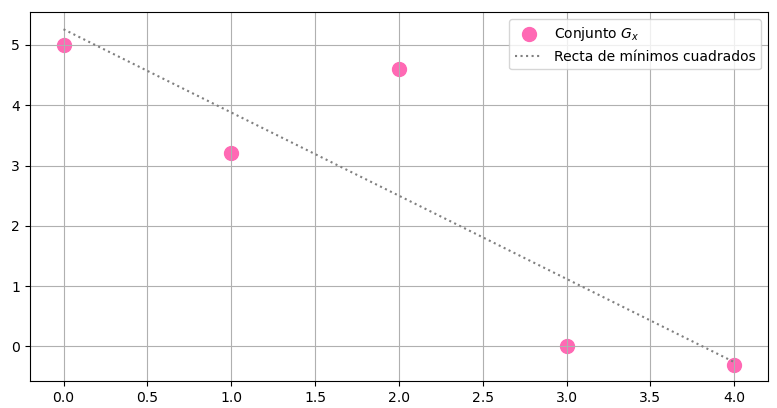
\includegraphics[scale = 0.3]{2Dic_1}
\end{figure}

\begin{figure}[h]
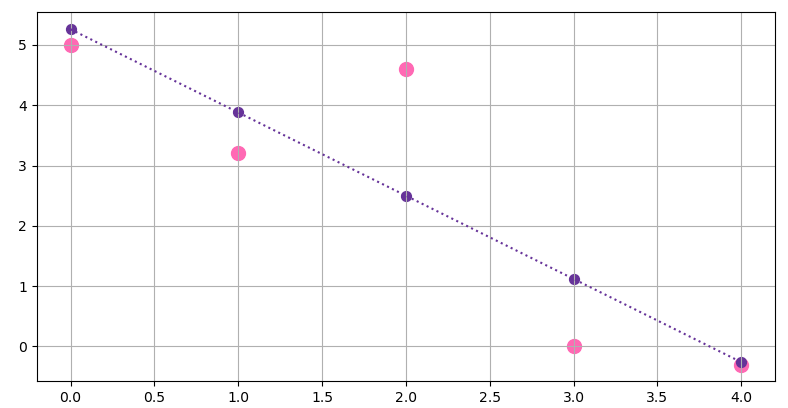
\includegraphics[scale = 0.3]{2Dic_2}
\end{figure}

\end{frame}

\begin{frame}
\begin{prop}
\label{prop: discretizacion recta minimos cuadrados}
Sea $n \geq 2$ y sea el conjunto de $n$ puntos del plano
\begin{equation}
\label{eq10: 10Dic}
\{(j, x_{j}): 0 \leq j \leq n-1 \}
\subseteq \IR^{2}.
\end{equation}
Si $x=(x_{j})_{j=0}^{n-1}$ es la señal cuya
gráfica $G_{x}$ coincide con el conjunto dado
en \eqref{eq10: 10Dic}, si
\begin{itemize}
\item $l_{min}: y= m_{0}t+ b_{0}$ es la recta obtenida 
aproximando los puntos del conjunto \eqref{eq10: 10Dic}
con el método de mínimos cuadrados, y

\item $l_{x}$ es la recta cuya versión discreta 
respecto a la malla uniforme $\cali{P}_{n}$
es $\Pi_{W_{n,1}}(x) \in \IR^{n}$, 

\end{itemize} 
entonces las rectas $l_{x}$ y $l_{min}$ coinciden.
\end{prop}
\end{frame}


\begin{frame}
\frametitle{Explicit formulas for the vectors $\cali{L}^{n,k}$}

For the task we use the formulas of the popular paper
\TODO{Neuman}, and we get that
\[
(\cali{L}_{m}^{n,k})_{m=0}^{n-1}
= \cali{L}^{n,k}
= (-1)^{k} \cdot 
\sqrt{\frac{(2k+1)(n-1)^{(k)}}{(n+k)^{(k+1)}}}
\left(
\suma{j=0}{k}{(-1)^{j}\binom{k}{j}\binom{k+j}{j}
\frac{m^{(j)}}{(n-1)^{(j)}}}
\right)_{m=0}^{n-1}.
\]
\end{frame}


\begin{frame}
\frametitle{Symmetries of the entries of the discrete polynomial $\cali{L}^{n,k}$}

\begin{figure}[h]
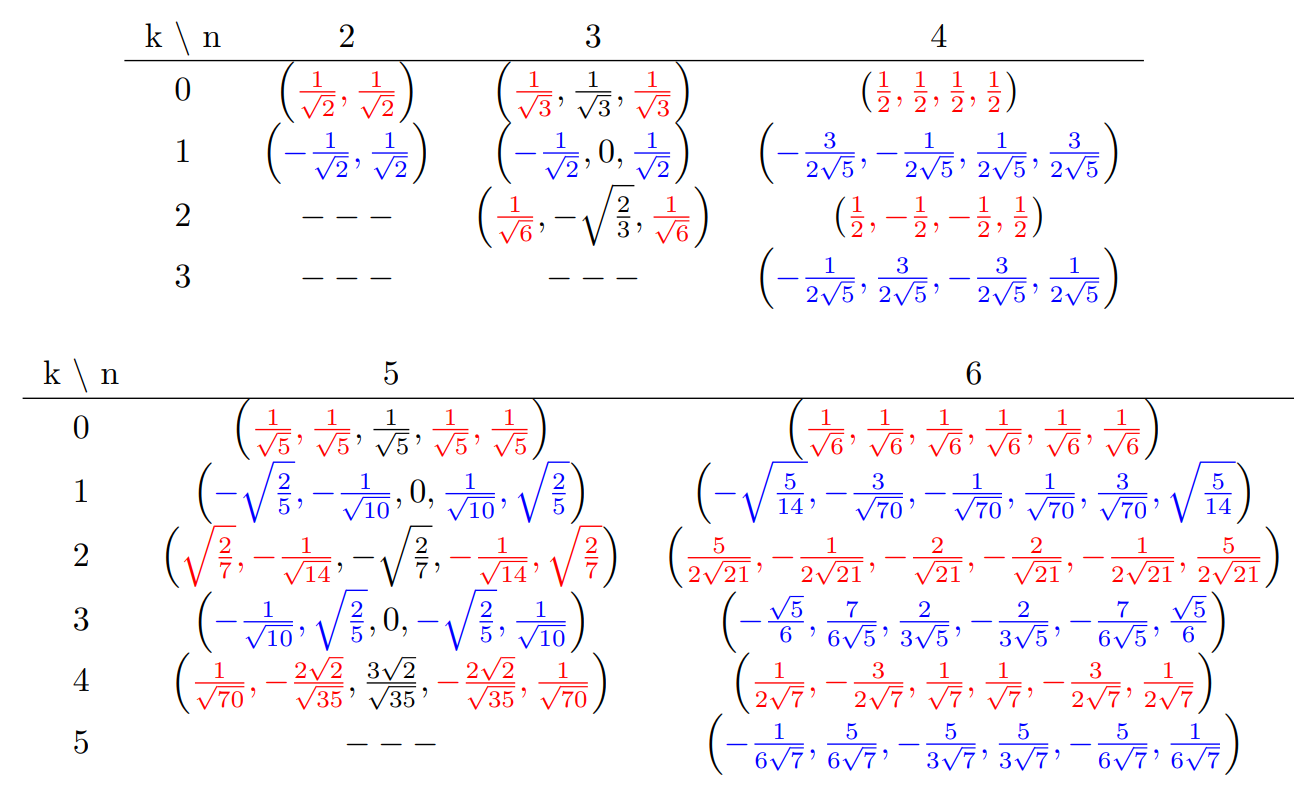
\includegraphics[scale = 0.3]{symm}
\end{figure}
\end{frame}


\begin{frame}
\begin{defi}
Let $n \geq 2$, $M := \lceil \frac{n}{2} \rfloor$. We define the
\textbf{space of $n-$dimensional symmetric signals} as
\[
S_{n, +} := \{ x = (x_{m})_{m=0}^{n-1} : \hspace{0.2cm} 
\forall 0 \leq m \leq M-1, \hspace{0.1cm} x_{m} = x_{n-m-1} \},
\]
and the \textbf{space of $n-$dimensional anti-symmetric signals} as
\[
S_{n, -} := \{ x = (x_{m})_{m=0}^{n-1} : \hspace{0.2cm} 
\forall 0 \leq m \leq M-1, \hspace{0.1cm} x_{m} = -x_{n-m-1} \},
\]
\end{defi}
\begin{figure}[h]
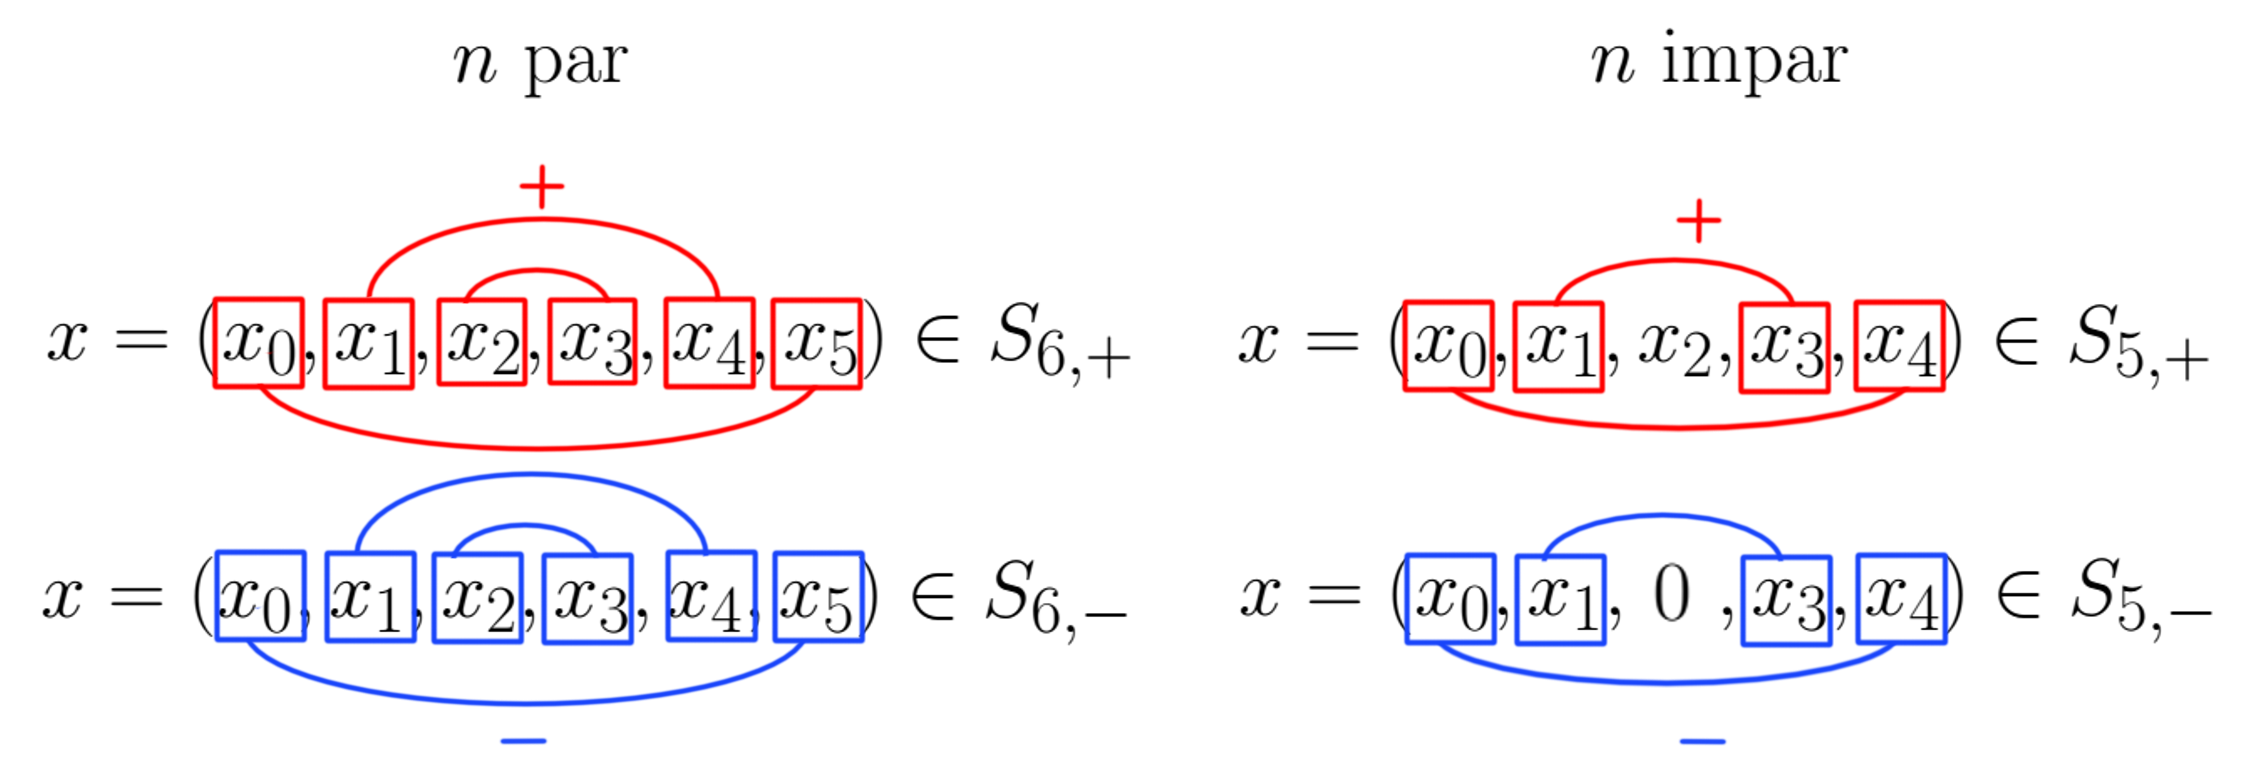
\includegraphics[scale = 0.4]{sim_antisim}
\end{figure}
\end{frame}




\begin{frame}
\begin{teo}
Let $n \geq 2$ , $0 \leq k \leq n-1$. Let 
$\cali{L}^{n,k} = (\cali{L}^{n,k}_{m})_{m=0}^{n-1}$ be
$n-$dimensional discrete Legendre polynomial of degree $k$. 
\begin{itemize}
	\item if $k$ is even, then $\cali{L}^{n,k} \in S_{n,+}$,
	\item if $k$ is odd, then $\cali{L}^{n,k} \in S_{n,-}$.
\end{itemize}
\end{teo}
\begin{figure}[h]
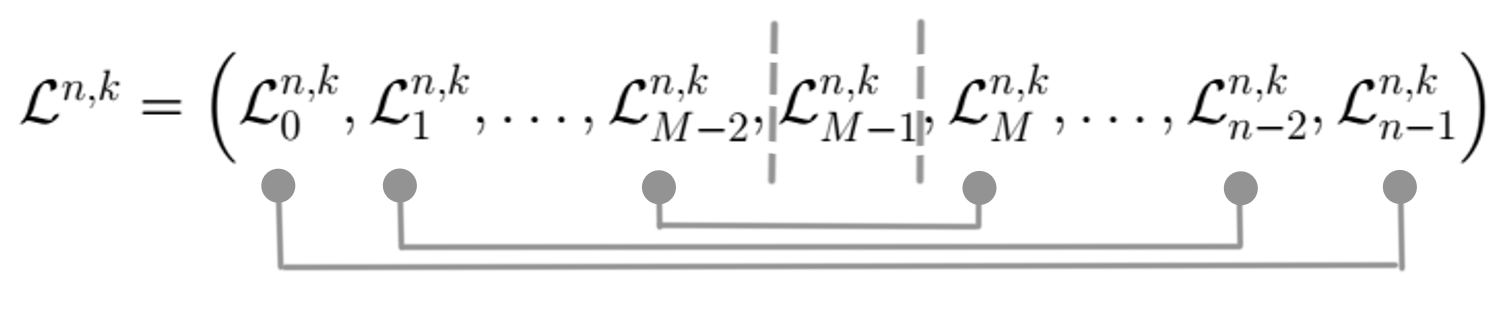
\includegraphics[scale = 0.5]{simetria1}
\end{figure}
\begin{figure}[h]
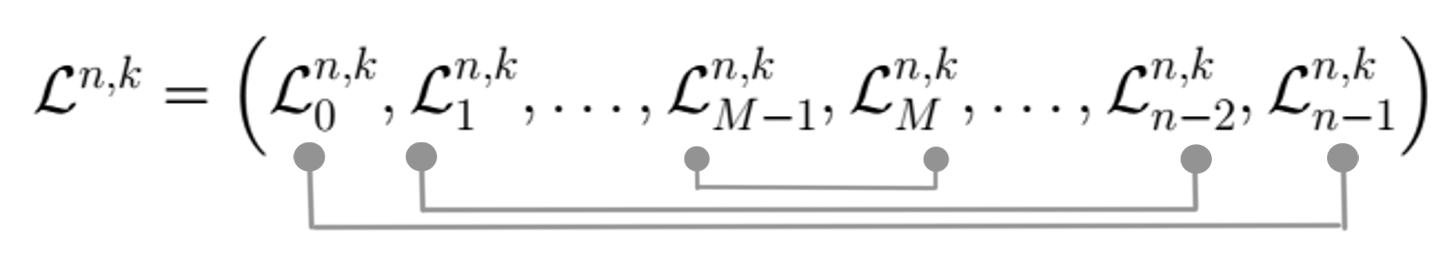
\includegraphics[scale = 0.5]{simetria2}
\end{figure}
\end{frame}

% ------------------------------------------------------------------------

\begin{frame}
\Huge{
\textbf{
Part Two: Spectral analysis
}}
\end{frame}

\begin{frame}
\frametitle{Motivation for performing a spectral analysis of the signals $\cali{L}^{n,k}$}
It's readily seen that the conditions of orthogonality imposed in the definition
of the vectors $\cali{L}^{n,k}$ force them to have more and more changes of sign as
$k$ increases.
\begin{figure}[h]
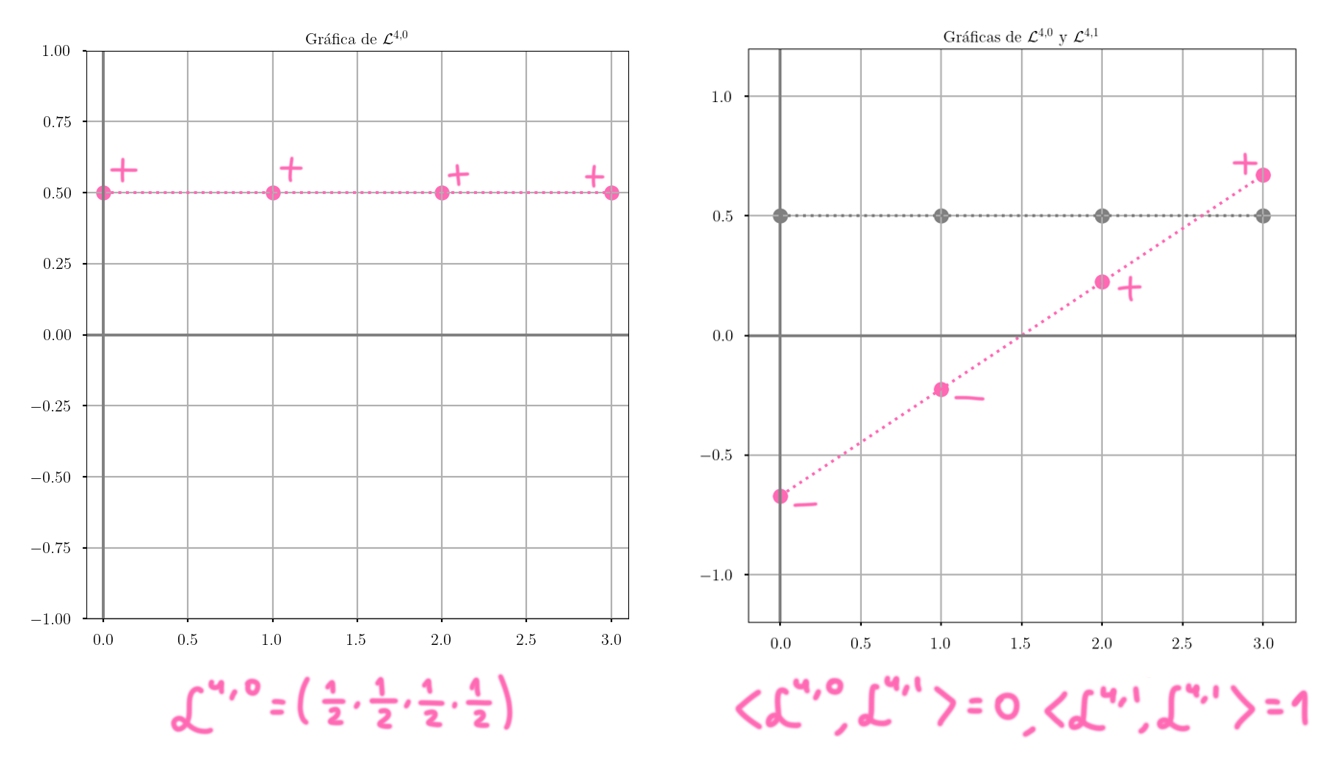
\includegraphics[scale = 0.6]{oscil1}
\end{figure}
\end{frame}

\begin{frame}
\begin{figure}[h]
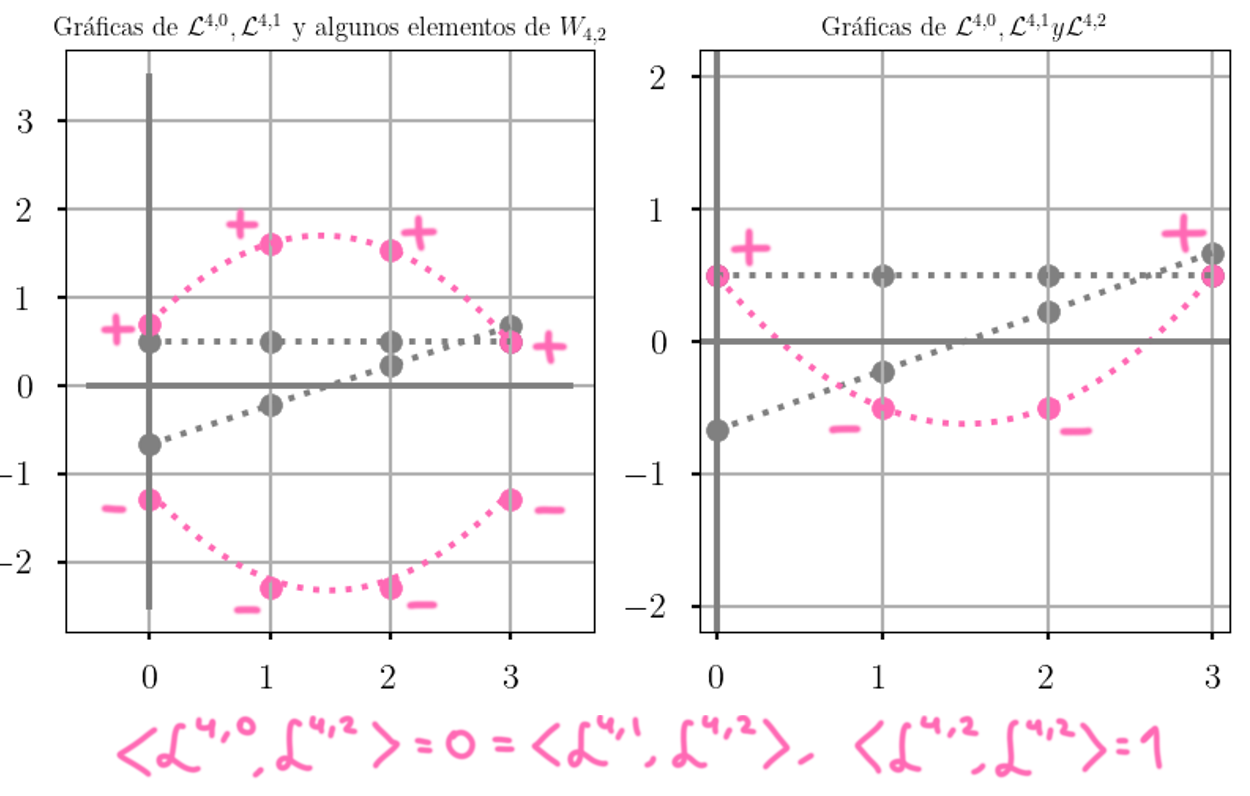
\includegraphics[scale = 0.9]{oscil2}
\end{figure}
\end{frame}

\begin{frame}
\begin{figure}[h]
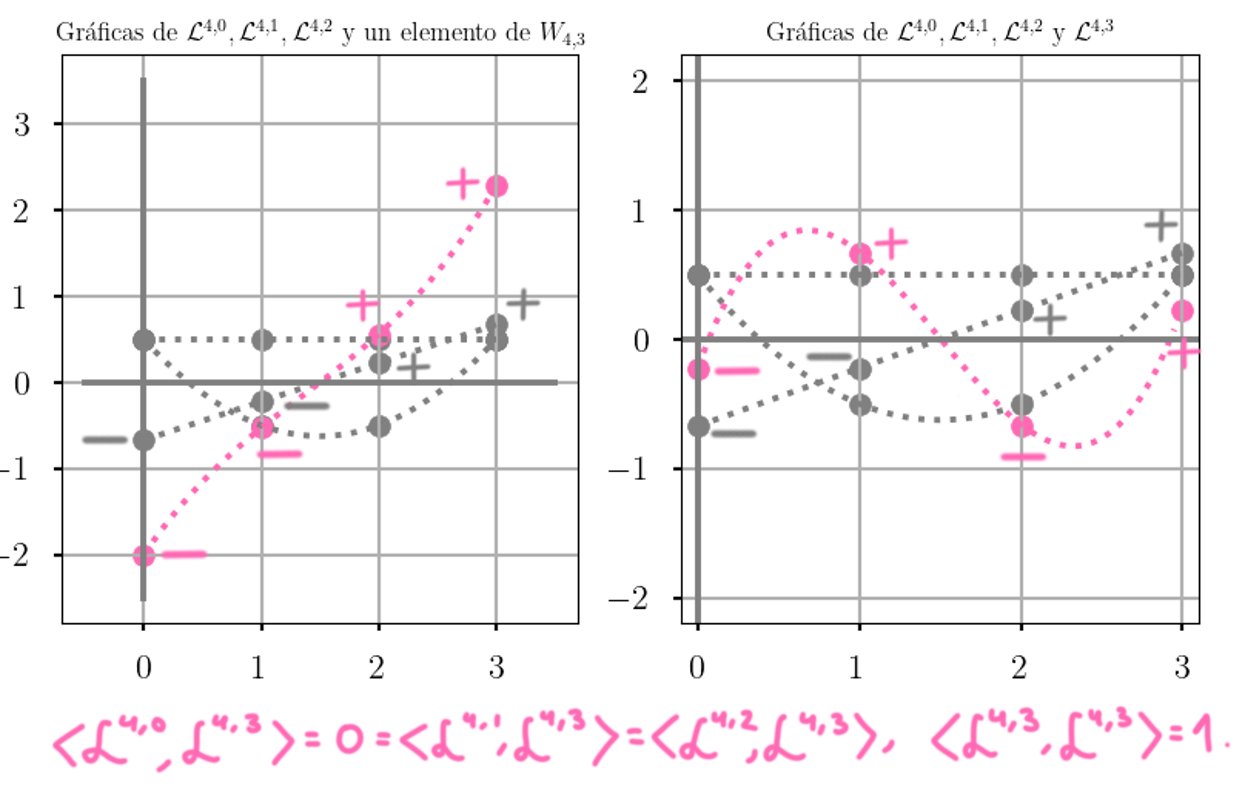
\includegraphics[scale = 0.9]{oscil3}
\end{figure}
\end{frame}


\begin{frame}
\frametitle{An hypothesis about the oscilation of the Legendre discrete polynomials}
\begin{figure}[h]
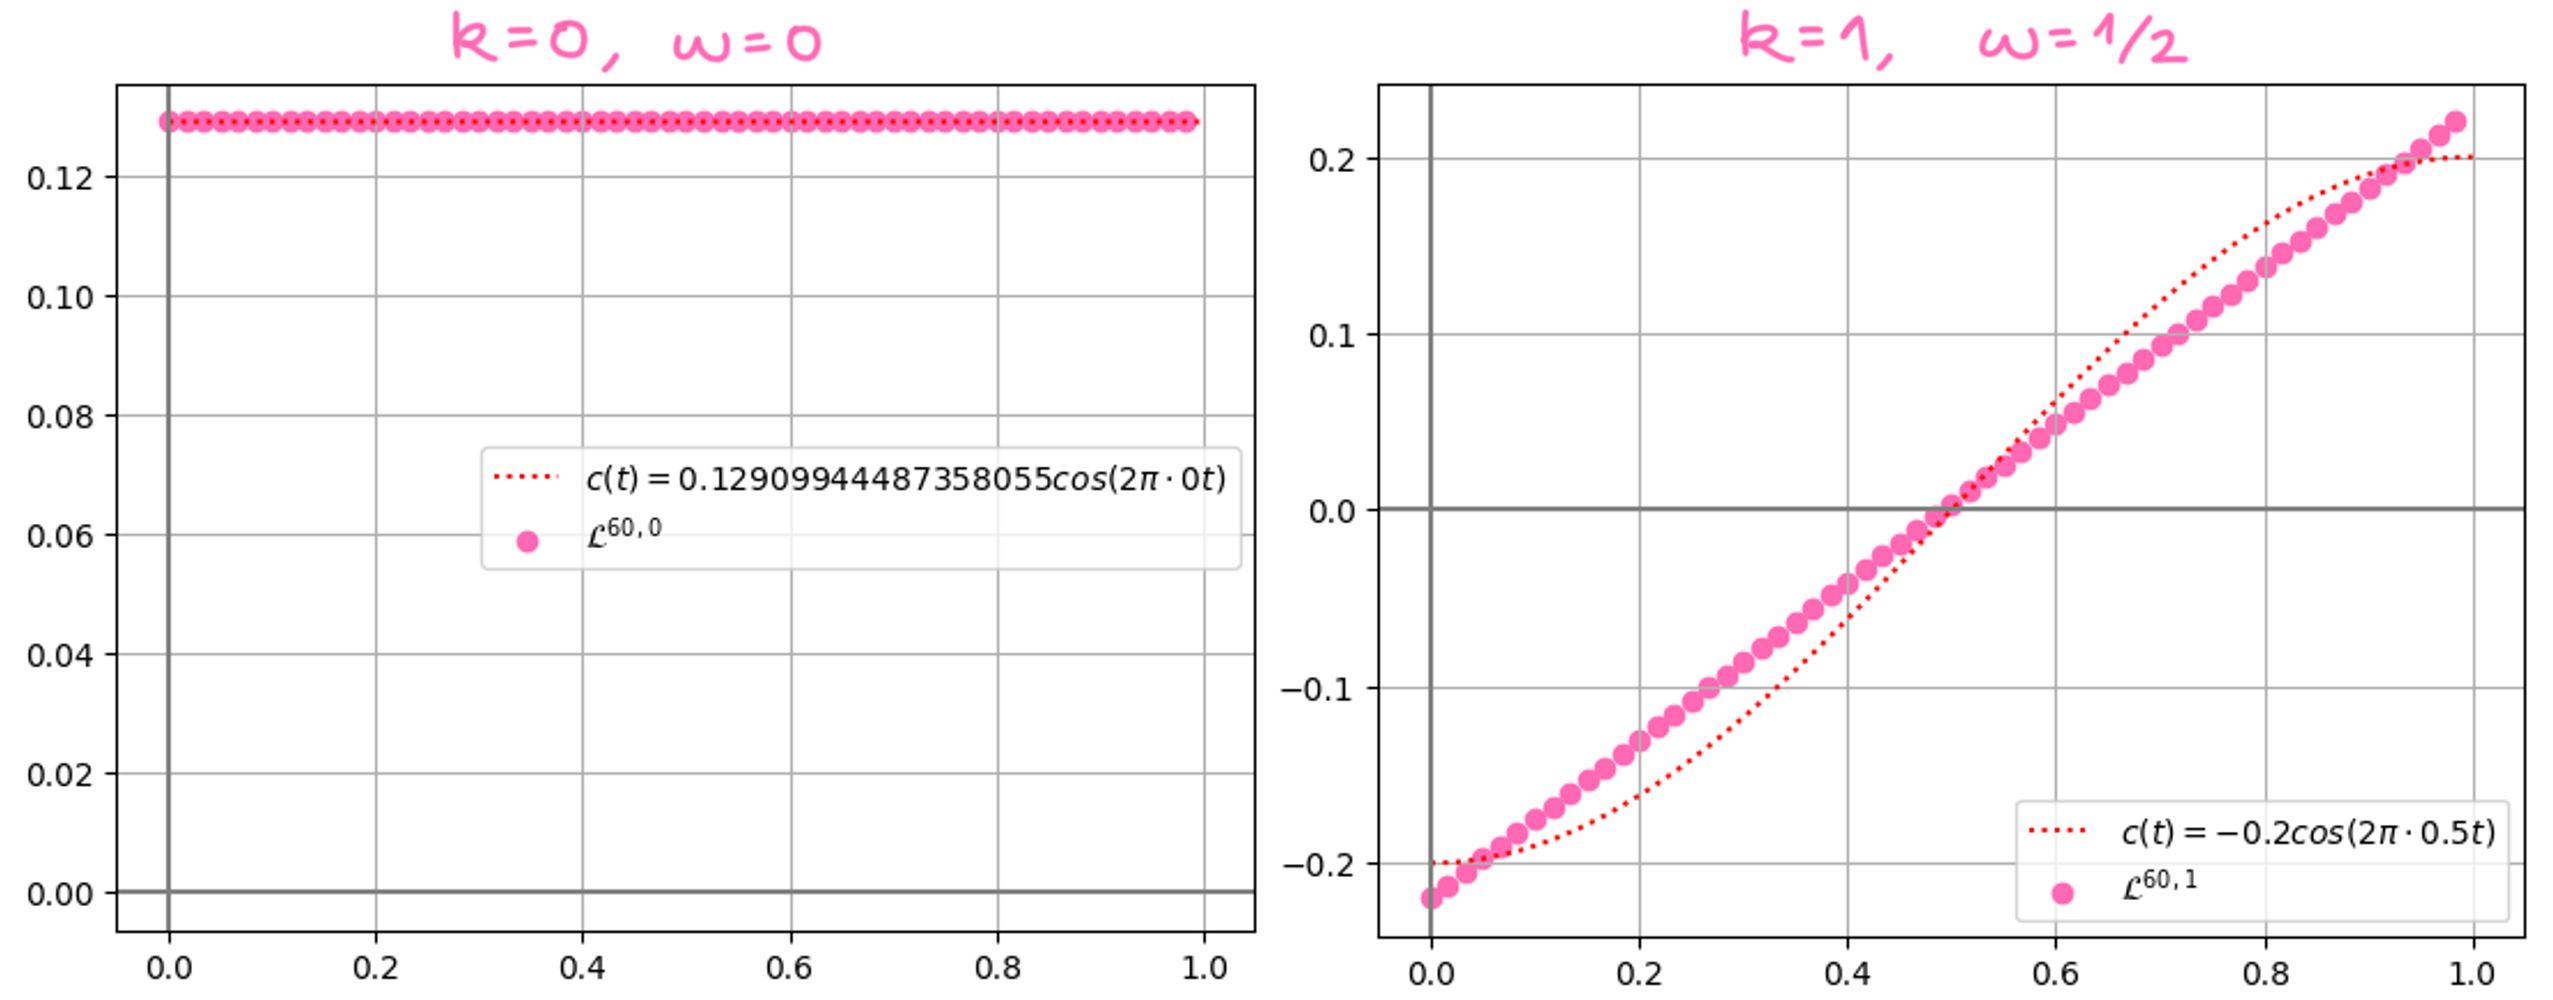
\includegraphics[scale = 0.5]{hip_0,1}
\end{figure}
\end{frame}



\begin{frame}
\begin{figure}[h]
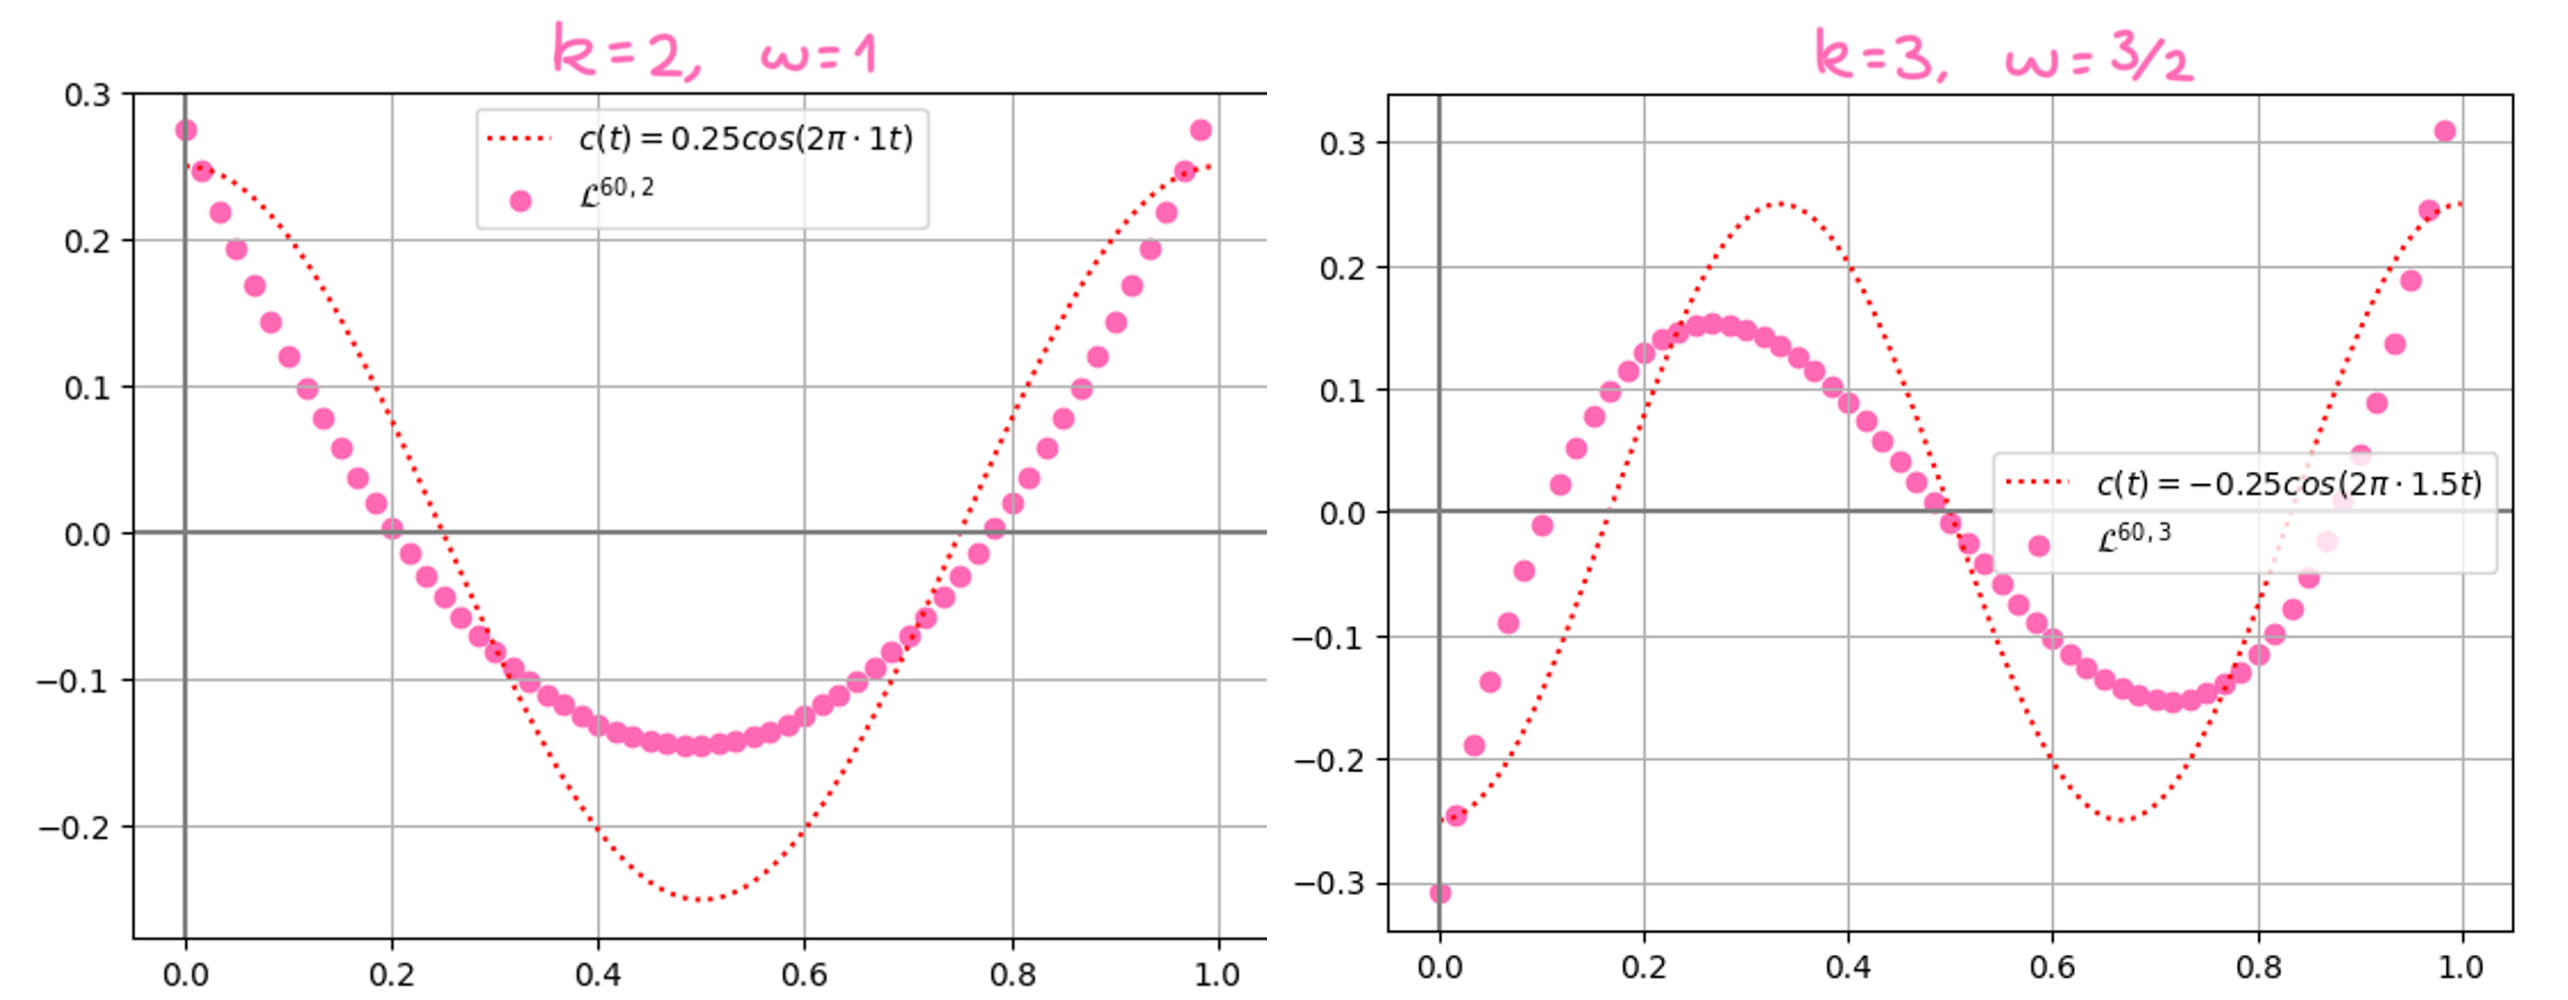
\includegraphics[scale = 0.5]{hip_2,3}
\end{figure}
\end{frame}


\begin{frame}
\begin{figure}[h]
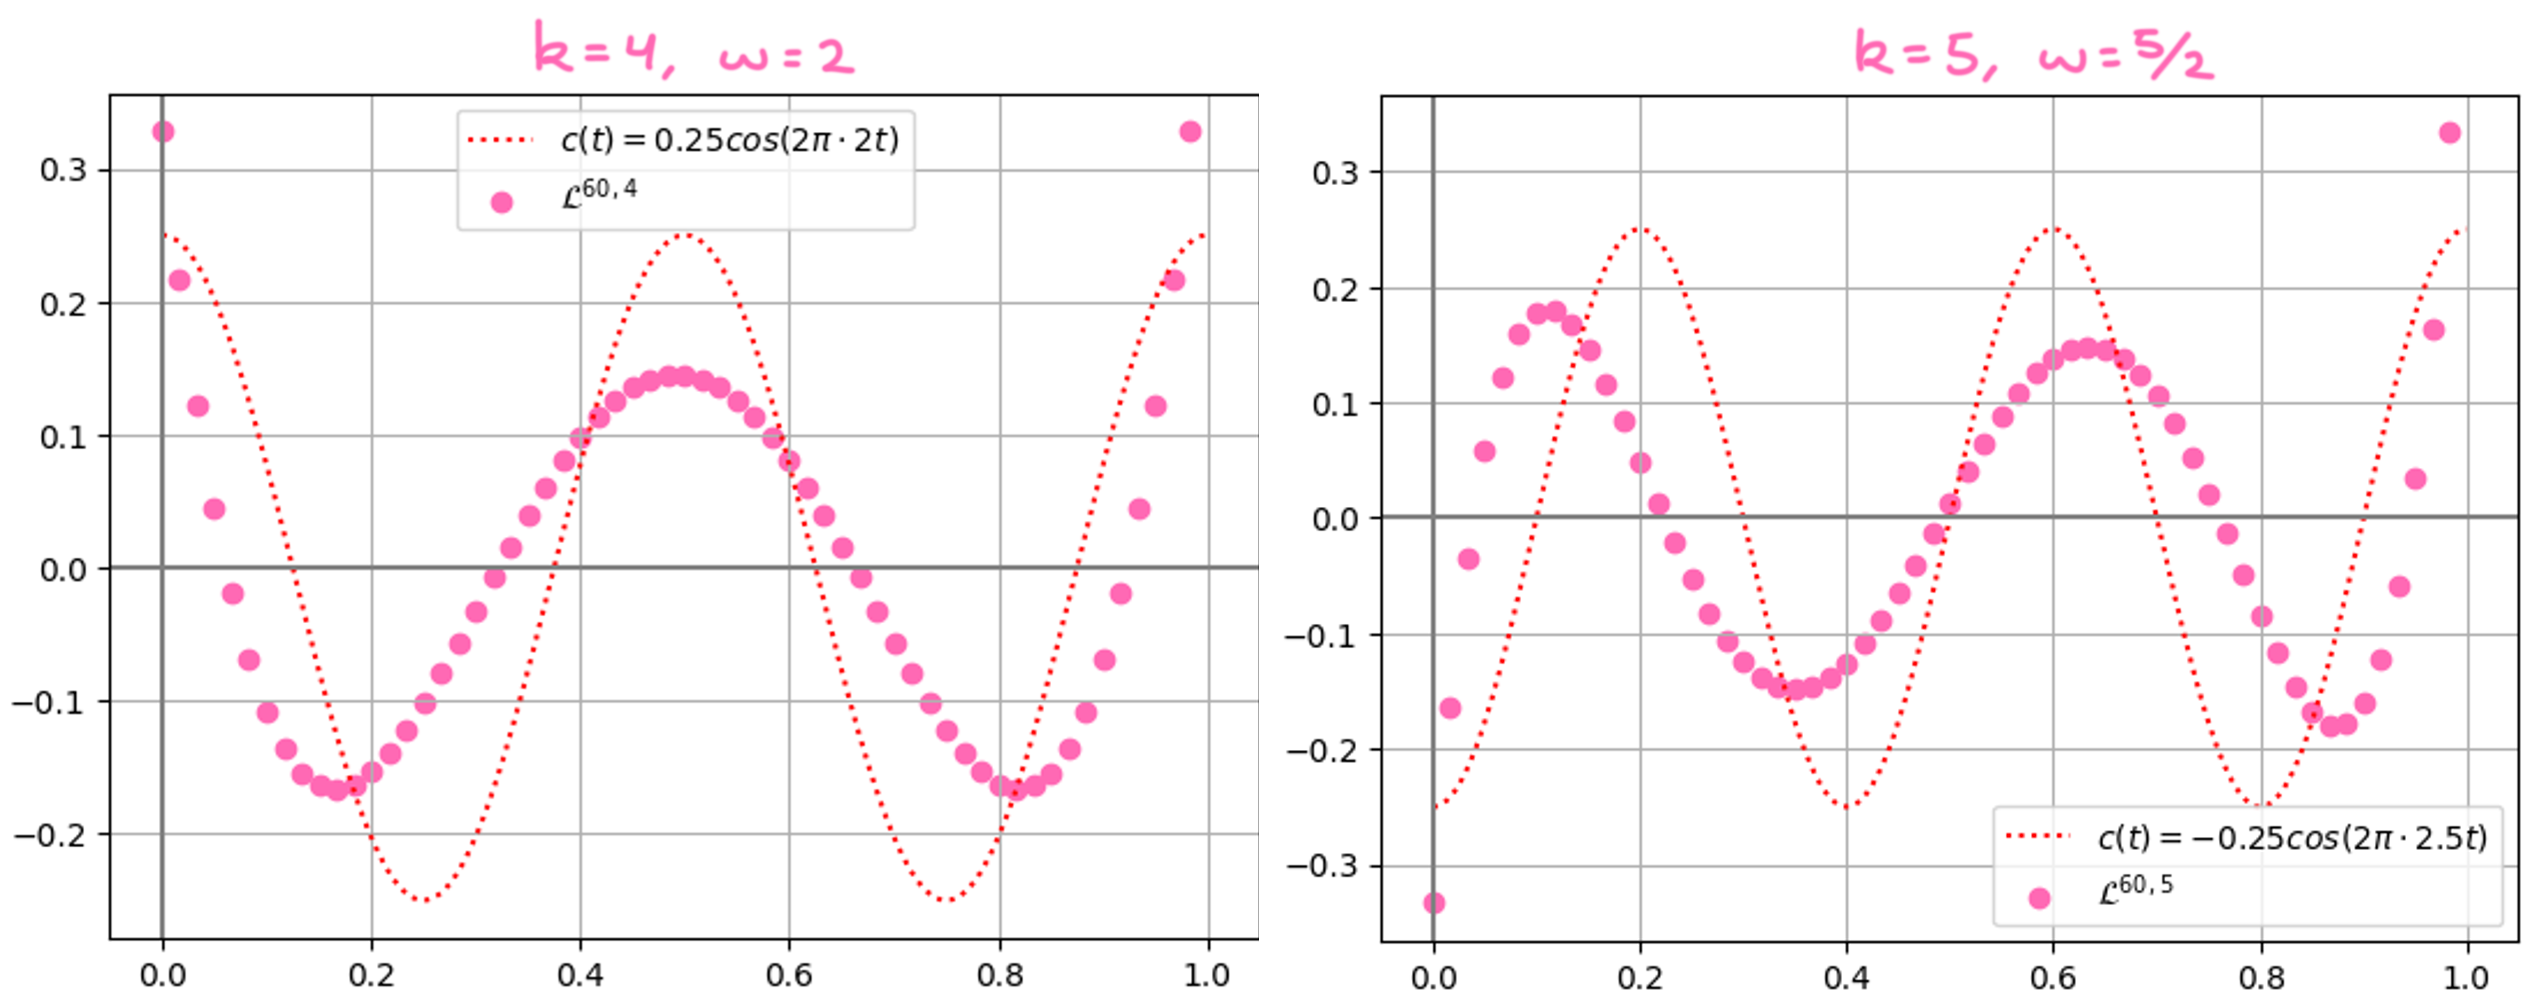
\includegraphics[scale = 0.5]{hip_4,5}
\end{figure}
\end{frame}

\begin{frame}
\begin{hip}
Let $n \geq 2$ and $0 \leq k \leq n-1$. If
$\cali{L}^{n,k}$ is the discrete Legendre polynomial of 
dimension $n$ and degree $k$, then the spectrum
of $\cali{L}^{n,k}$ is concentrated around the frequency
$k/2$.
\end{hip}

\begin{center}
\textbf{Which espectrum?}
\end{center}
\end{frame}




\begin{frame}
\frametitle{Classical spectrum using the DFT}
The idea is to represent a signal $x \in \IR^{n}$ in terms
of the orthonormal basis of frequencies 
$\cali{F}_{n}$, defined as
\TODO{eq}

\begin{figure}[h]
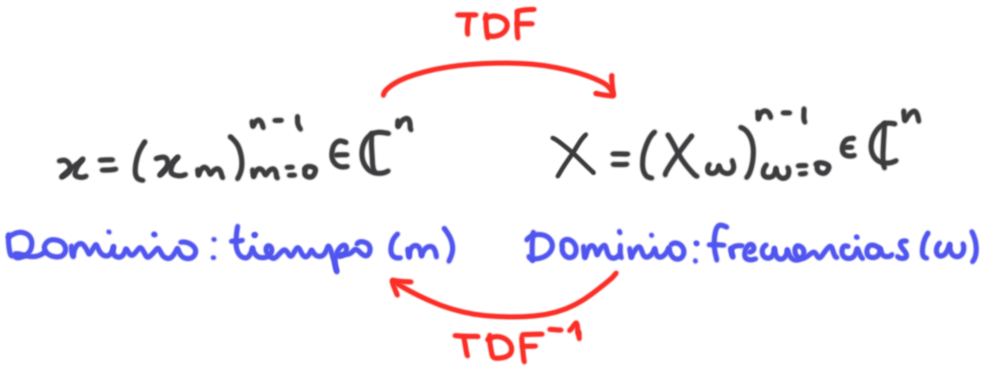
\includegraphics[scale = 0.6]{tiempo_freq}
\end{figure}
\end{frame}


\begin{frame}
\begin{defi}
\label{def: taus}
Let $n \geq 2$, $M = \lceil \frac{n}{2} \rceil $.
We define
	\[
	\tau_{n}(x, 0) := \frac{|\langle x, c_{n,0} \rangle|}{|| x ||} ,	
	\]
	and
	\[
	\forall 
	\hspace{0.1cm}	
	1 \leq \omega \leq M-1: \hspace{0.2cm} 
	\tau_{n}(x, \omega) := 
	\frac{\sqrt{
	\langle x, c_{n,\omega} \rangle^{2}+
	\langle x, s_{n,\omega} \rangle^{2}}}{||x||}.	
	\]	
	If $n$ is even, we also define
	\[
	\tau_{n}(x, M) := 
	\frac{ |\langle x, c_{n,M} \rangle| }{ ||x|| }.
	\]
\end{defi}
The function $T_{x}: Dom_{DFT, n} \longrightarrow [0,1]$
is the \textbf{spectrum of $x$} obtained using the DFT.
\end{frame}


\begin{frame}

To perform the analysis,
we would like to consider an arbitrary frequency $\omega$, not only
the integer frequencies taken into account in the DFT.

We want to 
\begin{enumerate}
	\item be able to chose a frequency $\omega \geq 0$ with respect to which
	compare the signal $x$, and
	
	\item once a frequency $\omega$ is fixed, being able to compute the 
	best phase to adjust the graph of $x$ with a sinusoid of frequency $\omega$.
\end{enumerate}
\end{frame}


\begin{frame}
\begin{figure}[h]
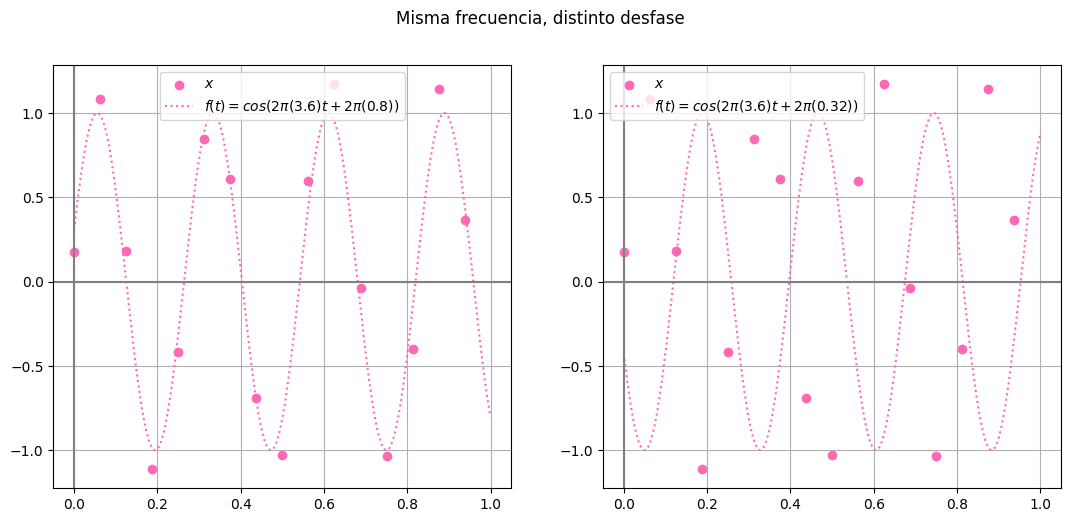
\includegraphics[scale = 0.4]{desfase_ejemplo}
\end{figure}
\end{frame}


\begin{frame}
\frametitle{Spectrum obtained measuring cosine distance to frequency spaces}

To overcome the problem stated above, we propose to make
an spectral analysis based in cosine similarity between the signal
$x$ and some \textbf{monofrecuency spaces}.

\end{frame}



\begin{frame}
\begin{defi}
Let $n \in \IN$,  $\omega>0$, $\phi \in [0,1[$.  
We will call any signal $x$ of the form

\begin{equation}
x =A \left(
cos \left(  2 \pi \omega m/n + 2 \pi \phi
\right)
\right)_{m=0}^{n-1},
\end{equation}

\noindent
where $A \in \IR$, an
\textbf{$n-$dimensional signal with pure frequency
$\omega$}. 
In this context, 
$\phi \in [0,1]$ will be called the \textbf{normalized phase}
of the signa, and $A \in \IR$ the \textbf{amplitude}.
\end{defi}

Note that any signal of the form 
$x =A \left(
sen \left(  2 \pi \omega m/n + 2 \pi \phi
\right)
\right)_{m=0}^{n-1}$ is also an 
$n-$dimensional signal with pure frequency
$\omega$.
\end{frame}

\begin{frame}
\begin{figure}[h]
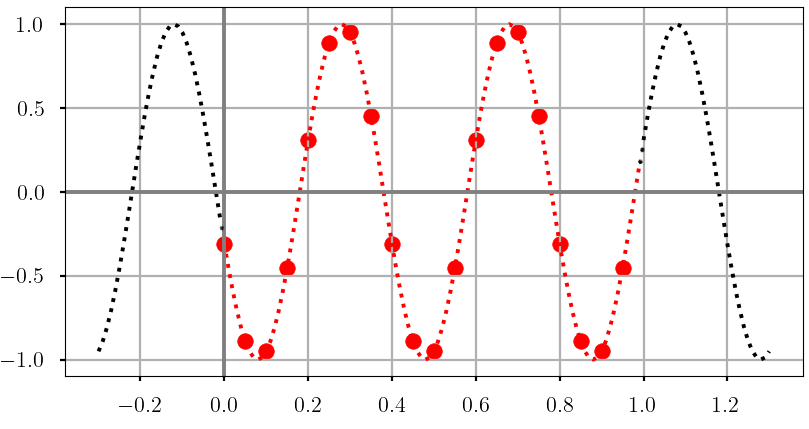
\includegraphics[scale = 0.4]{muestreo_coseno}
\end{figure}
\end{frame}

\begin{frame}
\frametitle{Monofrequency spaces}
Let $n \geq 2$ and $\omega \geq 0$. Let
\[
P_{n, \omega} := span \{ s_{n, \omega}, c_{n, \omega} \}.
\]

\begin{teo}
The subspace $P_{n, \omega}$ of $\IR^{n}$ is exactly the
set of $n-$dimensional signals with pure frequency $\omega$.
\end{teo}
$P_{n, \omega} \leq \IR^{n}$ is thus called the mono frequency space of 
dimension $n$ and frequency $\omega$.
\end{frame}

\begin{frame}
It makes sense then to use the cosine of the angle between
a signal $x$ and the space $P_{n, \omega}$ to asses how
present the frequency $\omega$ is in $x$.
\begin{figure}[h]
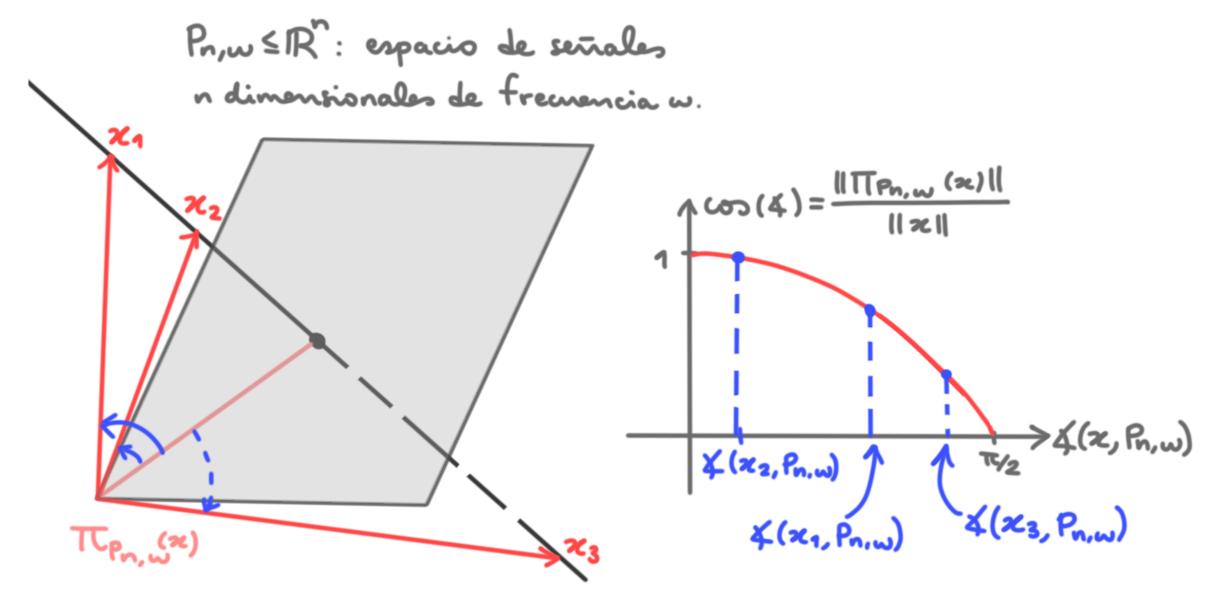
\includegraphics[scale = 1]{20Mar23_1}
\end{figure}
\end{frame}

\begin{frame}
\begin{defi}
\label{def: taus}
Let $n \geq 2$. For all $x \in \IR^{n}$ and $\omega \geq 0$
we define
	\[
	\sigma_{n}(x, \omega) := cos(\measuredangle(x, P_{n, \omega}))
	= \frac{|| \Pi_{P_{n, \omega}}(x) ||}{||x||}
	\]
\end{defi}
\end{frame}

\begin{frame}
\begin{prop}
\label{prop: producto punto entre f y g}
Fijados $n \geq 2$ y $\omega \geq 0$ con 
$\omega \not\in \frac{n}{2}\IZ$, 
el producto punto entre 
los vectores
$c_{n, \omega}$ y $s_{n, \omega}$, definidos 
\eqref{eq5: 19Marzo} y \eqref{eq6: 19Marzo}
respectivamente, es

\begin{equation}
\label{eq9: 19Marzo}
\langle c_{n, \omega} , s_{n, \omega} \rangle =
\frac{\xi_{n, w} \eta_{n, \omega}}{2} \cdot 
\frac{sen(2 \pi \omega)
sen(2 \pi \omega \left( 1- \frac{1}{n} \right))}{sen \left(2 \pi 
\frac{\omega}{n} \right)}
\end{equation}

Let $\Sigma_{x}: [0, \infty[ \longrightarrow [0,1]$
be defined
as \[
\Sigma_{x}(\omega) := \sigma_{n}(x, \omega).
\]

\end{prop}
\end{frame}


\begin{frame}
\frametitle{A computable formula for $\sigma_{n}(x, \omega)$ in terms of $x$.}
Sean $n \geq 2$, $\omega \geq 0$. 
Sea $\sigma_{n}(\cdot,\omega): \IR^{n} \longrightarrow [0,1]$
la función definida en \ref{def: final de sigmas}.
Para todo $x \in \IR^{n}-\{ 0 \}$
se tiene que
\begin{itemize}
	\item Si $\omega \not\in \frac{n}{2} \IZ$, entonces
	\begin{equation}
	\label{eq: pi ommm 1}
	 \Pi_{P_{n, \omega}}(x) = 
\frac{
\langle x, c_{n, \omega} \rangle - \langle c_{n, \omega}, s_{n, \omega} \rangle 
\langle x, s_{n, \omega} \rangle
}
{1-|\langle c_{n, \omega}, s_{n, \omega} \rangle |^{2}  }
c_{n, \omega} +
\frac{
\langle x, s_{n, \omega} \rangle - \langle c_{n, \omega}, s_{n, \omega} \rangle 
\langle x, c_{n, \omega} \rangle
}
{1-|\langle c_{n, \omega}, s_{n, \omega} \rangle |^{2}  }
s_{n, \omega}
	\end{equation}
	y 
	\begin{equation}
	\label{eq: coef sigma caso 1}
	\sigma_{n}(x, \omega) =
	\left(		  
		  \frac{\langle x, c_{n, \omega } \rangle^{2} +  \langle x, s_{n, \omega } \rangle^{2}	
	       -2  \langle x, c_{n, \omega } \rangle \langle x, s_{n, \omega } \rangle \langle c_{n, \omega }, s_{n, \omega } \rangle}{ || x ||^{2} \cdot
	       (1- \langle c_{n, \omega }, s_{n, \omega } \rangle^{2})}	  
\right) ^{1/2},
	\end{equation}
donde $c_{n, \omega}$ y $s_{n, \omega}$ son como en 
\eqref{eq5: 19Marzo} y \eqref{eq6: 19Marzo},  y
\end{itemize}
\end{frame}

\begin{frame}
\begin{itemize}
\item si $\omega \in \frac{n}{2} \IZ$, entonces 
\begin{equation}
\label{eq: pi ommm 2}
\Pi_{P_{n, \omega}}(x) = \langle x, c_{n, \omega} \rangle c_{n, \omega}
\end{equation}
y 
\begin{equation}
\label{eq: sfklmslsfl}
\sigma_{n}(x, \omega) = \frac{|\langle x, c_{n, \omega} \rangle |}{||x||},
\end{equation}
donde $c_{n, \omega}$ es como en \eqref{ec: 4: 23ap}.
\end{itemize}
\end{frame}

\begin{frame}
\frametitle{A formula for the amplitude and shift of the projection of a signal to a monofrecuency space}
\begin{teo}
\label{teo: amelie1}
\textbf{(Amplitud y desfase de la proyección de $x \in \IR^{n}$ al
espacio monofrecuencial $P_{n, \omega}$)}
Sean $n \geq 2$ y $\omega > 0$ con $\omega \not\in \frac{n}{2}\IZ$.
Si $P_{n, \omega}$ es el subespacio de $\IR^{n}$ definido como 
en \eqref{eq6: 23Ap}, entonces, para todo 
$x \in \IR^{n}$ no cero, se tiene que
\begin{equation}
\label{ec: desfase explicito 1}
\Pi_{P_{n, \omega}} (x) = A \cdot (
cos (2 \pi \omega t - 2 \pi \phi)
)_{t \in I_{n}} \in \IR^{n},
\end{equation}

\noindent
donde la amplitud $A$ es
\[
\sqrt{c^{2}+d^{2}},
\]
$c$ y $d$ son como en \eqref{eq4: 20Marzo} y 
\eqref{eq5: 20Marzo}, resp., y el desfase $\phi$ está 
dado por \eqref{eq: desfase phi 1}.
\end{teo}
\end{frame}

\begin{frame}
\begin{equation}
\label{eq4: 20Marzo}
c= \frac{
\langle x, c_{n, \omega} \rangle - \langle c_{n, \omega}, s_{n, \omega} \rangle
\langle x, s_{n, \omega} \rangle
}{1-\langle c_{n, \omega}, s_{n, \omega} \rangle^{2}} \xi_{n, \omega}
\end{equation}
y
\begin{equation}
\label{eq5: 20Marzo}
d= \frac{
\langle x, s_{n, \omega} \rangle - \langle c_{n, \omega}, s_{n, \omega} \rangle
\langle x, c_{n, \omega} \rangle
}{1-\langle c_{n, \omega}, s_{n, \omega} \rangle^{2}} \eta_{n, \omega}.
\end{equation}
\end{frame}

\begin{frame}
\begin{equation}
\label{eq: desfase phi 1}
\phi =
\begin{cases}
\frac{tan^{-1}(d/c) }{2 \pi}  \hspace{0.4cm}    \text{   si }   d, c > 0,  \\
\frac{tan^{-1}(d/c) + \pi }{2 \pi} \hspace{0.2cm}  \text{si }  d, c < 0
\text{ o } d<0, c>0, \\
\frac{tan^{-1}(d/c) + 2\pi }{2 \pi} \hspace{0.2cm}  \text{si }  d>0,  c < 0. 
\end{cases}
\end{equation}
\end{frame}


\begin{frame}
\begin{teo}
\label{teo: amelie2}
Sean $n \geq 2$ y $\omega > 0$ con $\omega \in \frac{n}{2}\IZ$.
Si $P_{n, \omega}$ es el subespacio de $\IR^{n}$ definido como 
en \eqref{eq0: 23Ap}, entonces, para todo 
$x \in \IR^{n}$ no cero, se tiene que
\begin{equation}
\label{ec: desfase explicito 2}
\Pi_{P_{n, \omega}} (x) = 
\frac{1}{\sqrt{n}} \langle x, c_{n, \omega} \rangle
\cdot (cos (2 \pi \omega t))_{t \in I_{n}} \in \IR^{n}.
\end{equation}
\end{teo}

\end{frame}


\begin{frame}
\frametitle{Some properties of $\Sigma_{x}$}
We fix a signal $x \in \IR^{n}-\{ 0\}$.
\begin{itemize}
	\item \textbf{n-th periodicity} For all $\omega >0$ and $K \in \IZ$,
	\[
	\Sigma_{x}(\omega) = \Sigma_{x}(\omega + Kn)
	\]
	\item \textbf{symmetry} For all $0 \leq \omega \leq n/2$, 
	\[
	\Sigma_{x}(\omega) = \Sigma_{x}(n-\omega).
	\]
\end{itemize}
\end{frame}

\begin{frame}
\begin{figure}[h]
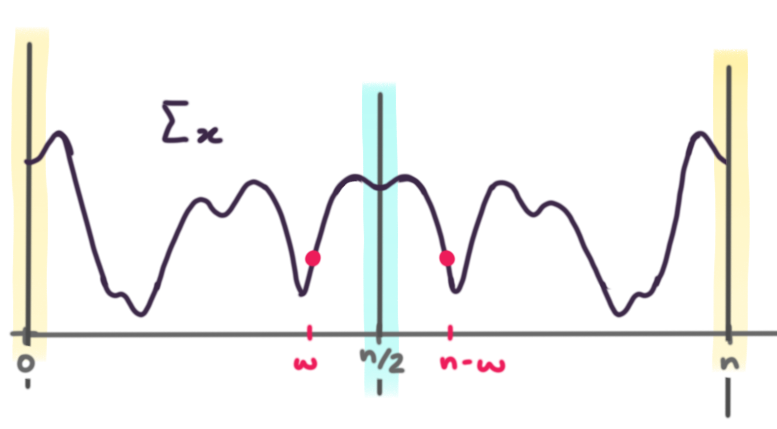
\includegraphics[scale = 1]{simetria_espectro}
\end{figure}

\begin{figure}[h]
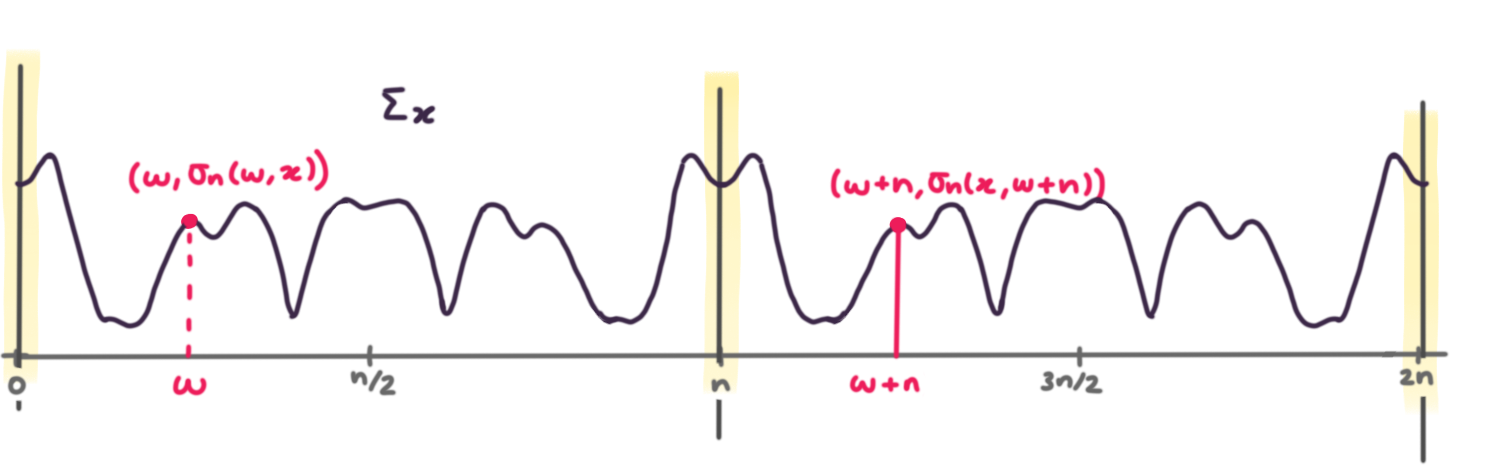
\includegraphics[scale = 0.8]{periodicidad_espectro}
\end{figure}

We can restrict $\Sigma_{x}$ to the frequency domain $[0, n/2]$
\end{frame}

\begin{frame}
\frametitle{Continuity of $\Sigma_{x}$}
Obviously $\Sigma_{x}$ is continuous in $]0, n/2[$. 
Using Taylor series expansions of the sine and cosine functions, we
were able to compute to sided limits in $0^{+}$ and $(n/2)^{-}$
of the function 
$\Sigma_{x}$.
\end{frame}

\begin{frame}
\begin{teo}
\label{teo: limite del espectro por cero}
Sean $n \geq 2$, $x \in \IR^{n}$.
Sea $\Sigma_{x}: [0, n/2] \rightarrow [0,1]$ 
como se definió en \eqref{eq: estudiando espectro}.
Se tiene que 
\begin{equation}
\label{eq: limite del espectro a cero}
\limite{\omega \rightarrow 0^{+}}{\Sigma_{x}(\omega)}
=
\left(
\frac{
2M_{0}(x)^{2}(2n-1)(n-1) + 12M_{1}(x)^{2} - 12M_{0}(x)M_{1}(x)(n-1)
}{
||x||^{2} (n-1)(n+1)n}
\right)^{1/2}
\end{equation}

y

\begin{equation}
\label{eq: limite del espectro a n medios}
\limite{\omega \rightarrow (n/2)^{-}}{\Sigma_{x}(\omega)}
= \limite{\omega \rightarrow 0^{+}}{\Sigma_{A_{n}(x)}(\omega)}.
\end{equation}
\end{teo}
\end{frame}

\begin{frame}
\begin{prop}
\label{prop: relacion limite cero con legendre}
Sean $n \geq 2$, $x \in \IR^{n}$,
$\Sigma_{x}$ el espectro de $x$.
Si $W_{n,1}$ es como en 
\eqref{espacios Wi}, el espacio
de los polinomios discretos de grado 
a lo más $1$ y dimensión $n$, entonces
\begin{equation}
\label{eq: limite por cero como angulo}
\limite{\omega \rightarrow 0^{+}}{
\Sigma_{x}(\omega)} = cos(\measuredangle(x, W_{n,1}))
\end{equation}
y
\begin{equation}
\label{eq: limite por cero como angulo}
\limite{\omega \rightarrow \frac{n}{2}^{-}}{
\Sigma_{x}(\omega)} = cos(\measuredangle(A_{n}(x), W_{n,1})).
\end{equation}
\end{prop}
\end{frame}

\begin{frame}
\begin{defi}
\label{def: espectro monofrecuenciales inicial}
\textbf{(Definición del espectro de una señal
basado en espacios monofrecuenciales)}
Sean $n \geq 2$, $x \in \IR^{n}$. \\

Si $x \neq 0$, definimos a su \textbf{espectro basado
en espacios monofrecuenciales} como la función 
$\Sigma_{x}: [0, n/2] \longrightarrow [0,1]$
definida como
\begin{align*}
\Sigma_{x}(\omega)= \begin{cases}
cos(\measuredangle(x, P_{n, \omega})) & 
\hspace{0.2cm} \textit{ si } \omega \in ]0, n/2[, \\
cos(\measuredangle(x, W_{n,1})) & \hspace{0.2cm} \textit{ si } \omega = 0, \\
cos(\measuredangle(A_{n}(x), W_{n,1})) & \hspace{0.2cm} \textit{ si } \omega = n/2.
\end{cases}
\end{align*}

Si $x = 0$, definimos su espectro como la 
función constante cero.
\end{defi}
\end{frame}


\begin{frame}
\begin{figure}[h]
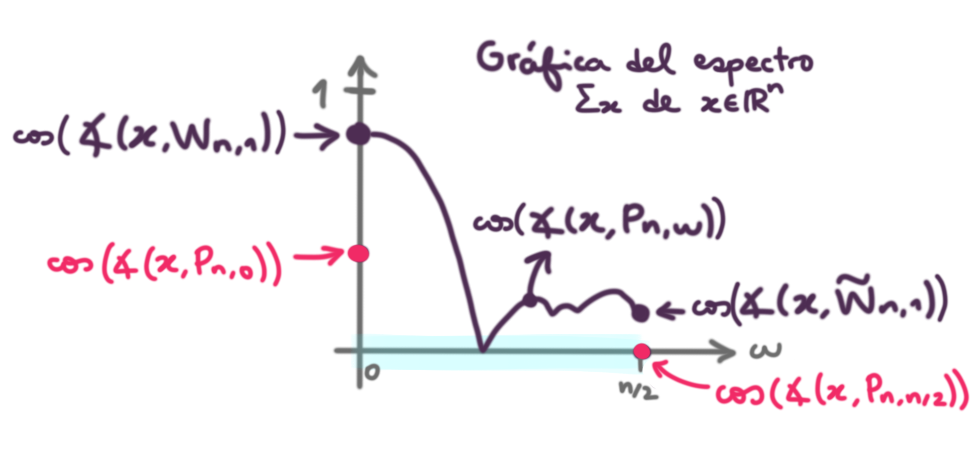
\includegraphics[scale = 1.4]{esp_ang}
\end{figure}
\end{frame}

\begin{frame}
\begin{figure}[h]
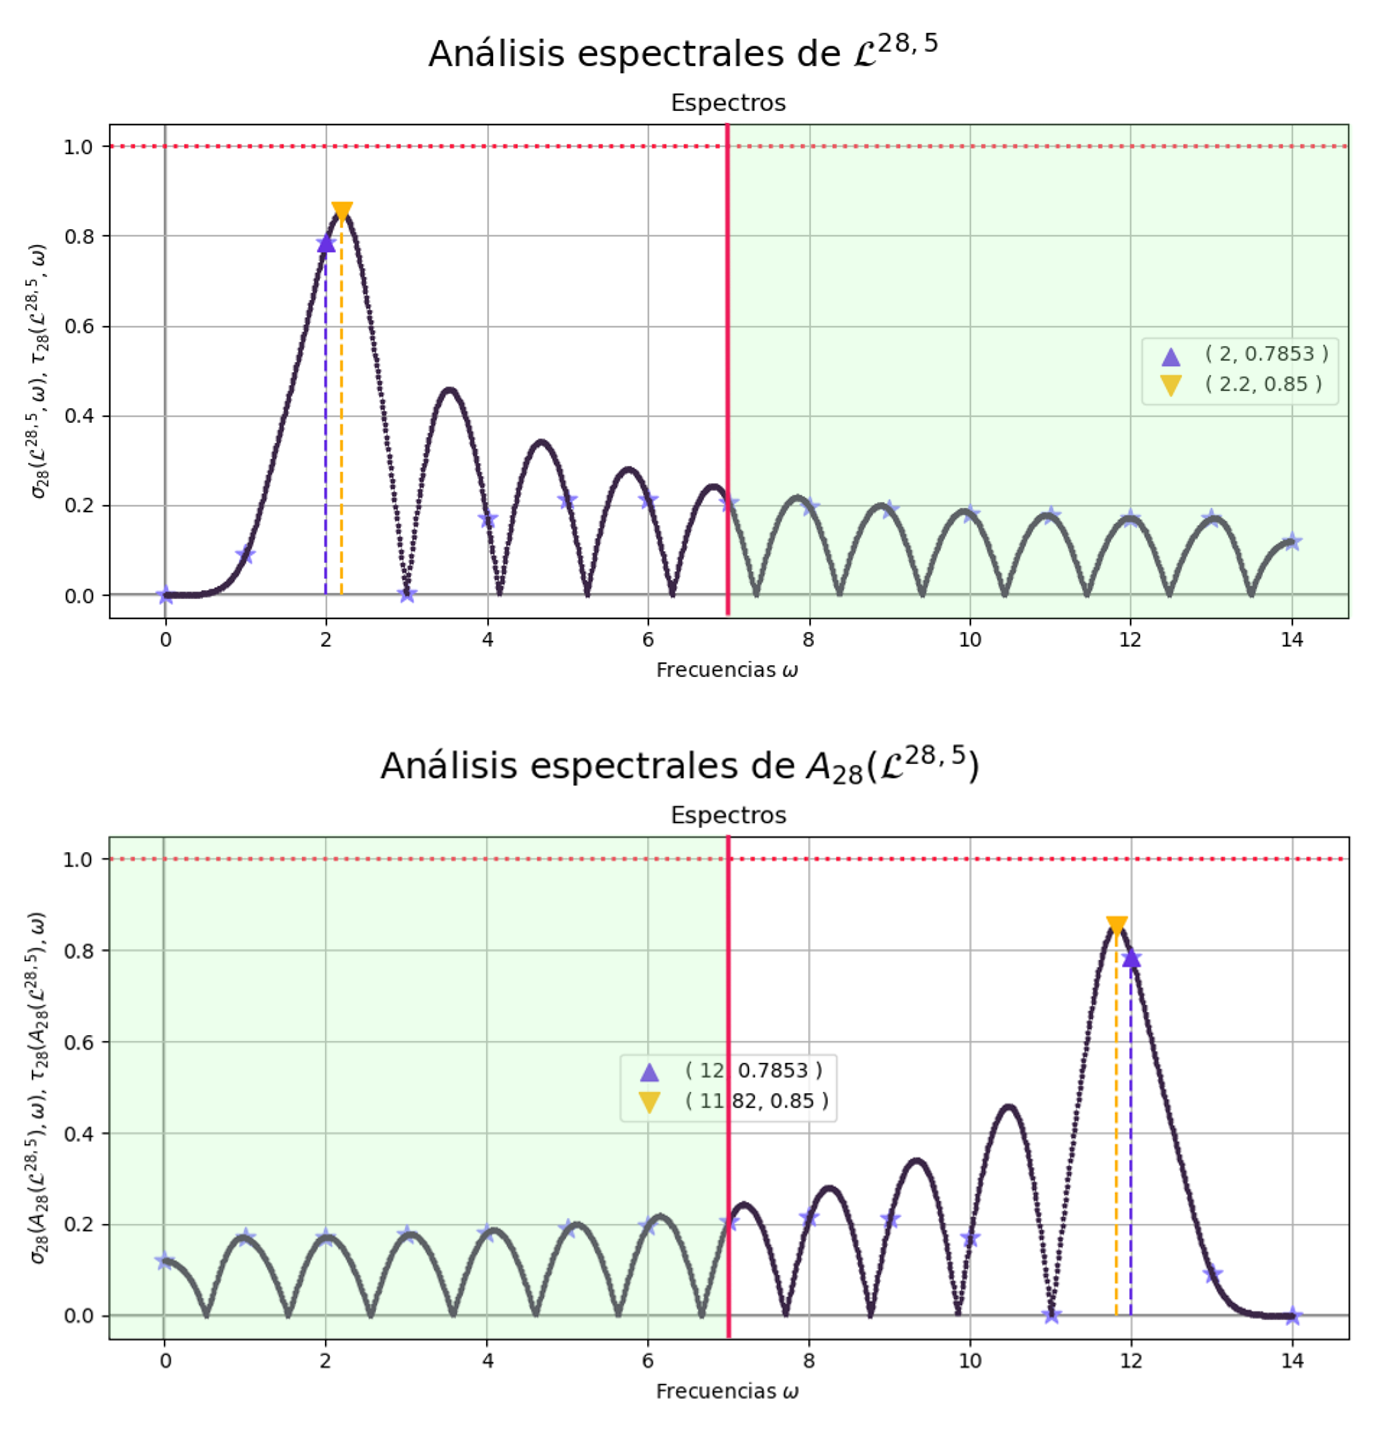
\includegraphics[scale = 0.7]{espectro_alternado}
\end{figure}
\end{frame}

\end{document}